\section{Пример решения задачи}

Рассмотрим пример задачи линейного программирования:

\subsection*{Исходная задача}
\begin{equation}
\begin{matrix}
    F(x) = -1x_{1} -1x_{2} -1x_{3} -1x_{4} + 2x_{5} \to \max \\
    \begin{cases}
    \begin{aligned}
        & 1x_{1} + 1x_{2} + 1x_{3} + 1x_{4} + 1x_{5} & = 1 \\
        & 1x_{1} -1x_{2} -1x_{3} + 1x_{4} + 1x_{5} & = 1 \\
        & 6x_{1} + 2x_{2} -1x_{3} + 1x_{4} -3x_{5} & \geq -1 \\
        & 1x_{1} -3x_{2} -5x_{3} -4x_{4} + 2x_{5} & \leq 1 \\
        & x_{1} \geq 0, \quad x_{2} \geq 0, \quad x_{3} \geq 0
    \end{aligned}
    \end{cases}
\end{matrix}
\end{equation}




\begin{enumerate}
\item Переменная $x_{4}$ заменена на: $x_{4} = \overline{x_{4}} - \overline{\overline{x_{4}}}, \quad \overline{x_{4}} \geq 0, \quad  \overline{\overline{x_{4}}} \geq 0$
\item Переменная $x_{5}$ заменена на: $x_{5} = \overline{x_{5}} - \overline{\overline{x_{5}}}, \quad \overline{x_{5}} \geq 0, \quad  \overline{\overline{x_{5}}} \geq 0$
\item Добавлена переменная $s_1,  s_1 \geq 0$
\item Добавлена переменная $s_2,  \quad s_2 \geq 0$
\end{enumerate}
\subsection*{Канонический вид}
\begin{equation}
\begin{matrix}
    F(x) = 1x_{1} + 1x_{2} + 1x_{3} + 1\overline{x_{4}} -2\overline{x_{5}} -1\overline{\overline{x_{4}}} + 2\overline{\overline{x_{5}}} \to \min \\
    \begin{cases}
    \begin{aligned}
        & 1x_{1} + 1x_{2} + 1x_{3} + 1\overline{x_{4}} + 1\overline{x_{5}} -1\overline{\overline{x_{4}}} -1\overline{\overline{x_{5}}} & = 1 \\
        & 1x_{1} -1x_{2} -1x_{3} + 1\overline{x_{4}} + 1\overline{x_{5}} -1\overline{\overline{x_{4}}} -1\overline{\overline{x_{5}}} & = 1 \\
        & -6x_{1} -2x_{2} + 1x_{3} -1\overline{x_{4}} + 3\overline{x_{5}} + 1\overline{\overline{x_{4}}} -3\overline{\overline{x_{5}}} + 1s_1 & = 1 \\
        & 1x_{1} -3x_{2} -5x_{3} -4\overline{x_{4}} + 2\overline{x_{5}} + 4\overline{\overline{x_{4}}} -2\overline{\overline{x_{5}}} + 1s_2 & = 1 \\
        & x_{1} \geq 0, \quad x_{2} \geq 0, \quad x_{3} \geq 0, \quad \overline{x_{4}} \geq 0, \quad \overline{x_{5}} \geq 0, \quad \overline{\overline{x_{4}}} \geq 0, \quad \overline{\overline{x_{5}}} \geq 0, \\
        & s_1 \geq 0, \quad s_2 \geq 0
    \end{aligned}
    \end{cases}
\end{matrix}
\end{equation}

\begin{itemize}
\subsection*{Поиск начального базиса методом введения искуственных переменных.}
\item Создана вспомогательная матрица $A_{aux}$:
$$\left[\begin{array}{ccccccccccccc}1 & 1 & 1 & 1 & 1 & -1 & -1 & 0 & 0 & 1 & 0 & 0 & 0\\1 & -1 & -1 & 1 & 1 & -1 & -1 & 0 & 0 & 0 & 1 & 0 & 0\\-6 & -2 & 1 & -1 & 3 & 1 & -3 & 1 & 0 & 0 & 0 & 1 & 0\\1 & -3 & -5 & -4 & 2 & 4 & -2 & 0 & 1 & 0 & 0 & 0 & 1\end{array}\right]$$
\item Определен вспомогательный вектор коэффициентов $c_{aux}$:
$$[0, 0, 0, 0, 0, 0, 0, 0, 0, 1, 1, 1, 1]$$
\item Определен базис:
$\lambda_1$
$\lambda_2$
$\lambda_3$
$\lambda_4$
\item Решение вспомогательной задачи с помощью симплекс-метода...
\subsection*{Итерация 1}
\begin{itemize}
\item \textbf{Базисные переменные:}
$\lambda_1$
$\lambda_2$
$\lambda_3$
$\lambda_4$
\item \textbf{Матрица базиса $B$:}
$\left[\begin{matrix}1 & 0 & 0 & 0\\0 & 1 & 0 & 0\\0 & 0 & 1 & 0\\0 & 0 & 0 & 1\end{matrix}\right]$
\item \textbf{Обратная матрица $B^{-1}$:}
$\left[\begin{matrix}1 & 0 & 0 & 0\\0 & 1 & 0 & 0\\0 & 0 & 1 & 0\\0 & 0 & 0 & 1\end{matrix}\right]$
\item \textbf{Значения базисных переменных $ x_i = B^{-1} \cdot b$:}
\begin{enumerate}
\item $\lambda_1 = 1$
\item $\lambda_2 = 1$
\item $\lambda_3 = 1$
\item $\lambda_4 = 1$
\end{enumerate}
\item \textbf{Вектор $c_b$:}
$[1, 1, 1, 1]$
\item \textbf{Вектор $y = c_B \cdot B^{-1}$:}
$[1, 1, 1, 1]$
\item \textbf{Оценки $\Delta = c - y \cdot A$:}
$[3, 5, 4, 3, -7, -3, 7, -1, -1, 0, 0, 0, 0]$
\item Минимальное значение у  $\Delta_{5} = -7$, который соотвествует переменной $\overline{x_{5}}$
\item \textbf{Направление $d = B^{-1} \cdot A_j$:}
$[1, 1, 3, 2]$
\item \textbf{Отношения $\theta = \frac{x_i}{d_i}$:}
\item $\theta_{1} = \frac{1}{1} = 1$
\item $\theta_{2} = \frac{1}{1} = 1$
\item $\theta_{3} = \frac{1}{3} = \frac{1}{3}$
\item $\theta_{4} = \frac{1}{2} = \frac{1}{2}$
\item Минимальное значение у  $\theta_{3} = \frac{1}{3}$, который соотвествует переменной $\lambda_3$
\item \textbf{Обновление базиса: $\lambda_3 \rightarrow \overline{x_{5}}$}
\end{itemize}
\newpage
\subsection*{Итерация 2}
\begin{itemize}
\item \textbf{Базисные переменные:}
$\lambda_1$
$\lambda_2$
$\overline{x_{5}}$
$\lambda_4$
\item \textbf{Матрица базиса $B$:}
$\left[\begin{matrix}1 & 0 & 1 & 0\\0 & 1 & 1 & 0\\0 & 0 & 3 & 0\\0 & 0 & 2 & 1\end{matrix}\right]$
\item \textbf{Обратная матрица $B^{-1}$:}
$\left[\begin{matrix}1 & 0 & - \frac{1}{3} & 0\\0 & 1 & - \frac{1}{3} & 0\\0 & 0 & \frac{1}{3} & 0\\0 & 0 & - \frac{2}{3} & 1\end{matrix}\right]$
\item \textbf{Значения базисных переменных $ x_i = B^{-1} \cdot b$:}
\begin{enumerate}
\item $\lambda_1 = \frac{2}{3}$
\item $\lambda_2 = \frac{2}{3}$
\item $\overline{x_{5}} = \frac{1}{3}$
\item $\lambda_4 = \frac{1}{3}$
\end{enumerate}
\item \textbf{Вектор $c_b$:}
$[1, 1, 0, 1]$
\item \textbf{Вектор $y = c_B \cdot B^{-1}$:}
$[1, 1, - \frac{4}{3}, 1]$
\item \textbf{Оценки $\Delta = c - y \cdot A$:}
$[-11, \frac{1}{3}, \frac{19}{3}, \frac{2}{3}, 0, - \frac{2}{3}, 0, \frac{4}{3}, -1, 0, 0, \frac{7}{3}, 0]$
\item Минимальное значение у  $\Delta_{1} = -11$, который соотвествует переменной $x_{1}$
\item \textbf{Направление $d = B^{-1} \cdot A_j$:}
$[3, 3, -2, 5]$
\item \textbf{Отношения $\theta = \frac{x_i}{d_i}$:}
\item $\theta_{1} = \frac{\frac{2}{3}}{3} = \frac{2}{9}$
\item $\theta_{2} = \frac{\frac{2}{3}}{3} = \frac{2}{9}$
\item $\theta_{3} = \infty$
\item $\theta_{4} = \frac{\frac{1}{3}}{5} = \frac{1}{15}$
\item Минимальное значение у  $\theta_{4} = \frac{1}{15}$, который соотвествует переменной $\lambda_4$
\item \textbf{Обновление базиса: $\lambda_4 \rightarrow x_{1}$}
\end{itemize}
\newpage
\subsection*{Итерация 3}
\begin{itemize}
\item \textbf{Базисные переменные:}
$\lambda_1$
$\lambda_2$
$\overline{x_{5}}$
$x_{1}$
\item \textbf{Матрица базиса $B$:}
$\left[\begin{matrix}1 & 0 & 1 & 1\\0 & 1 & 1 & 1\\0 & 0 & 3 & -6\\0 & 0 & 2 & 1\end{matrix}\right]$
\item \textbf{Обратная матрица $B^{-1}$:}
$\left[\begin{matrix}1 & 0 & \frac{1}{15} & - \frac{3}{5}\\0 & 1 & \frac{1}{15} & - \frac{3}{5}\\0 & 0 & \frac{1}{15} & \frac{2}{5}\\0 & 0 & - \frac{2}{15} & \frac{1}{5}\end{matrix}\right]$
\item \textbf{Значения базисных переменных $ x_i = B^{-1} \cdot b$:}
\begin{enumerate}
\item $\lambda_1 = \frac{7}{15}$
\item $\lambda_2 = \frac{7}{15}$
\item $\overline{x_{5}} = \frac{7}{15}$
\item $x_{1} = \frac{1}{15}$
\end{enumerate}
\item \textbf{Вектор $c_b$:}
$[1, 1, 0, 0]$
\item \textbf{Вектор $y = c_B \cdot B^{-1}$:}
$[1, 1, \frac{2}{15}, - \frac{6}{5}]$
\item \textbf{Оценки $\Delta = c - y \cdot A$:}
$[0, - \frac{10}{3}, - \frac{92}{15}, - \frac{20}{3}, 0, \frac{20}{3}, 0, - \frac{2}{15}, \frac{6}{5}, 0, 0, \frac{13}{15}, \frac{11}{5}]$
\item Минимальное значение у  $\Delta_{4} = - \frac{20}{3}$, который соотвествует переменной $\overline{x_{4}}$
\item \textbf{Направление $d = B^{-1} \cdot A_j$:}
$[\frac{10}{3}, \frac{10}{3}, - \frac{5}{3}, - \frac{2}{3}]$
\item \textbf{Отношения $\theta = \frac{x_i}{d_i}$:}
\item $\theta_{1} = \frac{\frac{7}{15}}{\frac{10}{3}} = \frac{7}{50}$
\item $\theta_{2} = \frac{\frac{7}{15}}{\frac{10}{3}} = \frac{7}{50}$
\item $\theta_{3} = \infty$
\item $\theta_{4} = \infty$
\item Минимальное значение у  $\theta_{1} = \frac{7}{50}$, который соотвествует переменной $\lambda_1$
\item \textbf{Обновление базиса: $\lambda_1 \rightarrow \overline{x_{4}}$}
\end{itemize}
\newpage
\subsection*{Итерация 4}
\begin{itemize}
\item \textbf{Базисные переменные:}
$\overline{x_{4}}$
$\lambda_2$
$\overline{x_{5}}$
$x_{1}$
\item \textbf{Матрица базиса $B$:}
$\left[\begin{matrix}1 & 0 & 1 & 1\\1 & 1 & 1 & 1\\-1 & 0 & 3 & -6\\-4 & 0 & 2 & 1\end{matrix}\right]$
\item \textbf{Обратная матрица $B^{-1}$:}
$\left[\begin{matrix}\frac{3}{10} & 0 & \frac{1}{50} & - \frac{9}{50}\\-1 & 1 & 0 & 0\\\frac{1}{2} & 0 & \frac{1}{10} & \frac{1}{10}\\\frac{1}{5} & 0 & - \frac{3}{25} & \frac{2}{25}\end{matrix}\right]$
\item \textbf{Значения базисных переменных $ x_i = B^{-1} \cdot b$:}
\begin{enumerate}
\item $\overline{x_{4}} = \frac{7}{50}$
\item $\lambda_2 = 0$
\item $\overline{x_{5}} = \frac{7}{10}$
\item $x_{1} = \frac{4}{25}$
\end{enumerate}
\item \textbf{Вектор $c_b$:}
$[0, 1, 0, 0]$
\item \textbf{Вектор $y = c_B \cdot B^{-1}$:}
$[-1, 1, 0, 0]$
\item \textbf{Оценки $\Delta = c - y \cdot A$:}
$[0, 2, 2, 0, 0, 0, 0, 0, 0, 2, 0, 1, 1]$
\item \textbf{Оптимальное решение найдено.}
\item \textbf{Решение $x$:}
$[\frac{4}{25}, 0, 0, \frac{7}{50}, \frac{7}{10}, 0, 0, 0, 0, 0, 0, 0, 0]$
\end{itemize}
\item Результат решения вспомогательной задачи $x_{aux}$:
$[\frac{4}{25}, 0, 0, \frac{7}{50}, \frac{7}{10}, 0, 0, 0, 0, 0, 0, 0, 0]$
\item Обновленный базис:
$\overline{x_{4}}$
$\overline{x_{5}}$
$x_{1}$
$x_{2}$
\newpage
\item Решение основной задачи с помощью симплекс-метода...
\subsection*{Итерация 1}
\begin{itemize}
\item \textbf{Базисные переменные:}
$\overline{x_{4}}$
$\overline{x_{5}}$
$x_{1}$
$x_{2}$
\item \textbf{Матрица базиса $B$:}
$\left[\begin{matrix}1 & 1 & 1 & 1\\1 & 1 & 1 & -1\\-1 & 3 & -6 & -2\\-4 & 2 & 1 & -3\end{matrix}\right]$
\item \textbf{Обратная матрица $B^{-1}$:}
$\left[\begin{matrix}- \frac{1}{10} & \frac{2}{5} & \frac{1}{50} & - \frac{9}{50}\\\frac{1}{2} & 0 & \frac{1}{10} & \frac{1}{10}\\\frac{1}{10} & \frac{1}{10} & - \frac{3}{25} & \frac{2}{25}\\\frac{1}{2} & - \frac{1}{2} & 0 & 0\end{matrix}\right]$
\item \textbf{Значения базисных переменных $ x_i = B^{-1} \cdot b$:}
\begin{enumerate}
\item $\overline{x_{4}} = \frac{7}{50}$
\item $\overline{x_{5}} = \frac{7}{10}$
\item $x_{1} = \frac{4}{25}$
\item $x_{2} = 0$
\end{enumerate}
\item \textbf{Вектор $c_b$:}
$[1, -2, 1, 1]$
\item \textbf{Вектор $y = c_B \cdot B^{-1}$:}
$[- \frac{1}{2}, 0, - \frac{3}{10}, - \frac{3}{10}]$
\item \textbf{Оценки $\Delta = c - y \cdot A$:}
$[0, 0, \frac{3}{10}, 0, 0, 0, 0, \frac{3}{10}, \frac{3}{10}]$
\item \textbf{Оптимальное решение найдено.}
\item \textbf{Решение $x$:}
$[\frac{4}{25}, 0, 0, \frac{7}{50}, \frac{7}{10}, 0, 0, 0, 0]$
\end{itemize}
\end{itemize}
\section*{Выводы и результаты}
\begin{itemize}
\item \textbf{Оптимальные значения переменных:}
\item $x_{1} = \frac{4}{25}$
\item $x_{2} = 0$
\item $x_{3} = 0$
\item $x_{4} = \frac{7}{50}$
\item $x_{5} = \frac{7}{10}$
\item \textbf{Значение целевой функции:} $z = \frac{11}{10}$
\end{itemize}




\newpage
\subsection*{Двойственная задача}
\begin{equation}
\begin{matrix}
    F(x) = 1x_1 + 1x_2 + 1x_3 + 1x_4 \to \min \\
    \begin{cases}
    \begin{aligned}
        & 1x_1 + 1x_2 -6x_3 + 1x_4 & \geq -1 \\
        & 1x_1 -1x_2 -2x_3 -3x_4 & \geq -1 \\
        & 1x_1 -1x_2 + 1x_3 -5x_4 & \geq -1 \\
        & 1x_1 + 1x_2 -1x_3 -4x_4 & \geq -1 \\
        & 1x_1 + 1x_2 + 3x_3 + 2x_4 & \geq 2 \\
        & -1x_1 -1x_2 + 1x_3 + 4x_4 & \geq 1 \\
        & -1x_1 -1x_2 -3x_3 -2x_4 & \geq -2 \\
        & x_3 \geq 0, \quad x_4 \geq 0
    \end{aligned}
    \end{cases}
\end{matrix}
\end{equation}




\begin{enumerate}
\item Переменная $x_1$ заменена на: $x_1 = \overline{x_1} - \overline{\overline{x_1}}, \quad \overline{x_1} \geq 0, \quad  \overline{\overline{x_1}} \geq 0$
\item Переменная $x_2$ заменена на: $x_2 = \overline{x_2} - \overline{\overline{x_2}}, \quad \overline{x_2} \geq 0, \quad  \overline{\overline{x_2}} \geq 0$
\item Добавлена переменная $s_1,  s_1 \geq 0$
\item Добавлена переменная $s_2,  s_2 \geq 0$
\item Добавлена переменная $s_3,  s_3 \geq 0$
\item Добавлена переменная $s_4,  s_4 \geq 0$
\item Добавлена переменная $s_5,  s_5 \geq 0$
\item Добавлена переменная $s_6,  s_6 \geq 0$
\item Добавлена переменная $s_7,  s_7 \geq 0$
\end{enumerate}
\subsection*{Канонический вид}
\begin{equation}
\begin{matrix}
    F(x) = 1\overline{x_1} + 1\overline{x_2} + 1x_3 + 1x_4 -1\overline{\overline{x_1}} -1\overline{\overline{x_2}} \to \min \\
    \begin{cases}
    \begin{aligned}
        & -1\overline{x_1} -1\overline{x_2} + 6x_3 -1x_4 + 1\overline{\overline{x_1}} + 1\overline{\overline{x_2}} + 1s_1 & = 1 \\
        & -1\overline{x_1} + 1\overline{x_2} + 2x_3 + 3x_4 + 1\overline{\overline{x_1}} -1\overline{\overline{x_2}} + 1s_2 & = 1 \\
        & -1\overline{x_1} + 1\overline{x_2} -1x_3 + 5x_4 + 1\overline{\overline{x_1}} -1\overline{\overline{x_2}} + 1s_3 & = 1 \\
        & -1\overline{x_1} -1\overline{x_2} + 1x_3 + 4x_4 + 1\overline{\overline{x_1}} + 1\overline{\overline{x_2}} + 1s_4 & = 1 \\
        & 1\overline{x_1} + 1\overline{x_2} + 3x_3 + 2x_4 -1\overline{\overline{x_1}} -1\overline{\overline{x_2}} -1s_5 & = 2 \\
        & -1\overline{x_1} -1\overline{x_2} + 1x_3 + 4x_4 + 1\overline{\overline{x_1}} + 1\overline{\overline{x_2}} -1s_6 & = 1 \\
        & 1\overline{x_1} + 1\overline{x_2} + 3x_3 + 2x_4 -1\overline{\overline{x_1}} -1\overline{\overline{x_2}} + 1s_7 & = 2 \\
        & \overline{x_1} \geq 0, \quad \overline{x_2} \geq 0, \quad x_3 \geq 0, \quad x_4 \geq 0, \quad \overline{\overline{x_1}} \geq 0, \quad \overline{\overline{x_2}} \geq 0, \\
        &  s_1 \geq 0, \quad s_2 \geq 0, \quad s_3 \geq 0, \quad s_4 \geq 0, \quad s_5 \geq 0, \quad s_6 \geq 0, \quad s_7 \geq 0
    \end{aligned}
    \end{cases}
\end{matrix}
\end{equation}




\begin{itemize}
\subsection*{Поиск начального базиса методом введения искуственных переменных.}
\item Создана вспомогательная матрица $A_{aux}$:
$$\left[\begin{array}{cccccccccccccccccccc}-1 & -1 & 6 & -1 & 1 & 1 & 1 & 0 & 0 & 0 & 0 & 0 & 0 & 1 & 0 & 0 & 0 & 0 & 0 & 0\\-1 & 1 & 2 & 3 & 1 & -1 & 0 & 1 & 0 & 0 & 0 & 0 & 0 & 0 & 1 & 0 & 0 & 0 & 0 & 0\\-1 & 1 & -1 & 5 & 1 & -1 & 0 & 0 & 1 & 0 & 0 & 0 & 0 & 0 & 0 & 1 & 0 & 0 & 0 & 0\\-1 & -1 & 1 & 4 & 1 & 1 & 0 & 0 & 0 & 1 & 0 & 0 & 0 & 0 & 0 & 0 & 1 & 0 & 0 & 0\\1 & 1 & 3 & 2 & -1 & -1 & 0 & 0 & 0 & 0 & -1 & 0 & 0 & 0 & 0 & 0 & 0 & 1 & 0 & 0\\-1 & -1 & 1 & 4 & 1 & 1 & 0 & 0 & 0 & 0 & 0 & -1 & 0 & 0 & 0 & 0 & 0 & 0 & 1 & 0\\1 & 1 & 3 & 2 & -1 & -1 & 0 & 0 & 0 & 0 & 0 & 0 & 1 & 0 & 0 & 0 & 0 & 0 & 0 & 1\end{array}\right]$$
\item Определен вспомогательный вектор коэффициентов $c_{aux}$:
$$[0, 0, 0, 0, 0, 0, 0, 0, 0, 0, 0, 0, 0, 1, 1, 1, 1, 1, 1, 1]$$
\item Определен базис:
$\lambda_1$
$\lambda_2$
$\lambda_3$
$\lambda_4$
$\lambda_5$
$\lambda_6$
$\lambda_7$
\item Решение вспомогательной задачи с помощью симплекс-метода...
\subsection*{Итерация 1}
\begin{itemize}
\item \textbf{Базисные переменные:}
$\lambda_1$
$\lambda_2$
$\lambda_3$
$\lambda_4$
$\lambda_5$
$\lambda_6$
$\lambda_7$
\item \textbf{Матрица базиса $B$:}
$\left[\begin{matrix}1 & 0 & 0 & 0 & 0 & 0 & 0\\0 & 1 & 0 & 0 & 0 & 0 & 0\\0 & 0 & 1 & 0 & 0 & 0 & 0\\0 & 0 & 0 & 1 & 0 & 0 & 0\\0 & 0 & 0 & 0 & 1 & 0 & 0\\0 & 0 & 0 & 0 & 0 & 1 & 0\\0 & 0 & 0 & 0 & 0 & 0 & 1\end{matrix}\right]$
\item \textbf{Обратная матрица $B^{-1}$:}
$\left[\begin{matrix}1 & 0 & 0 & 0 & 0 & 0 & 0\\0 & 1 & 0 & 0 & 0 & 0 & 0\\0 & 0 & 1 & 0 & 0 & 0 & 0\\0 & 0 & 0 & 1 & 0 & 0 & 0\\0 & 0 & 0 & 0 & 1 & 0 & 0\\0 & 0 & 0 & 0 & 0 & 1 & 0\\0 & 0 & 0 & 0 & 0 & 0 & 1\end{matrix}\right]$
\item \textbf{Значения базисных переменных $ x_i = B^{-1} \cdot b$:}
\begin{enumerate}
\item $\lambda_1 = 1$
\item $\lambda_2 = 1$
\item $\lambda_3 = 1$
\item $\lambda_4 = 1$
\item $\lambda_5 = 2$
\item $\lambda_6 = 1$
\item $\lambda_7 = 2$
\end{enumerate}
\item \textbf{Вектор $c_b$:}
$[1, 1, 1, 1, 1, 1, 1]$
\item \textbf{Вектор $y = c_B \cdot B^{-1}$:}
$[1, 1, 1, 1, 1, 1, 1]$
\item \textbf{Оценки $\Delta = c - y \cdot A$:}
$[3, -1, -15, -19, -3, 1, -1, -1, -1, -1, 1, 1, -1, 0, 0, 0, 0, 0, 0, 0]$
\item Минимальное значение у  $\Delta_{4} = -19$, который соотвествует переменной $x_4$
\item \textbf{Направление $d = B^{-1} \cdot A_j$:}
$[-1, 3, 5, 4, 2, 4, 2]$
\item \textbf{Отношения $\theta = \frac{x_i}{d_i}$:}
\item $\theta_{1} = \infty$
\item $\theta_{2} = \frac{1}{3} = \frac{1}{3}$
\item $\theta_{3} = \frac{1}{5} = \frac{1}{5}$
\item $\theta_{4} = \frac{1}{4} = \frac{1}{4}$
\item $\theta_{5} = \frac{2}{2} = 1$
\item $\theta_{6} = \frac{1}{4} = \frac{1}{4}$
\item $\theta_{7} = \frac{2}{2} = 1$
\item Минимальное значение у  $\theta_{3} = \frac{1}{5}$, который соотвествует переменной $\lambda_3$
\item \textbf{Обновление базиса: $\lambda_3 \rightarrow x_4$}
\end{itemize}
\newpage
\subsection*{Итерация 2}
\begin{itemize}
\item \textbf{Базисные переменные:}
$\lambda_1$
$\lambda_2$
$x_4$
$\lambda_4$
$\lambda_5$
$\lambda_6$
$\lambda_7$
\item \textbf{Матрица базиса $B$:}
$\left[\begin{matrix}1 & 0 & -1 & 0 & 0 & 0 & 0\\0 & 1 & 3 & 0 & 0 & 0 & 0\\0 & 0 & 5 & 0 & 0 & 0 & 0\\0 & 0 & 4 & 1 & 0 & 0 & 0\\0 & 0 & 2 & 0 & 1 & 0 & 0\\0 & 0 & 4 & 0 & 0 & 1 & 0\\0 & 0 & 2 & 0 & 0 & 0 & 1\end{matrix}\right]$
\item \textbf{Обратная матрица $B^{-1}$:}
$\left[\begin{matrix}1 & 0 & \frac{1}{5} & 0 & 0 & 0 & 0\\0 & 1 & - \frac{3}{5} & 0 & 0 & 0 & 0\\0 & 0 & \frac{1}{5} & 0 & 0 & 0 & 0\\0 & 0 & - \frac{4}{5} & 1 & 0 & 0 & 0\\0 & 0 & - \frac{2}{5} & 0 & 1 & 0 & 0\\0 & 0 & - \frac{4}{5} & 0 & 0 & 1 & 0\\0 & 0 & - \frac{2}{5} & 0 & 0 & 0 & 1\end{matrix}\right]$
\item \textbf{Значения базисных переменных $ x_i = B^{-1} \cdot b$:}
\begin{enumerate}
\item $\lambda_1 = \frac{6}{5}$
\item $\lambda_2 = \frac{2}{5}$
\item $x_4 = \frac{1}{5}$
\item $\lambda_4 = \frac{1}{5}$
\item $\lambda_5 = \frac{8}{5}$
\item $\lambda_6 = \frac{1}{5}$
\item $\lambda_7 = \frac{8}{5}$
\end{enumerate}
\item \textbf{Вектор $c_b$:}
$[1, 1, 0, 1, 1, 1, 1]$
\item \textbf{Вектор $y = c_B \cdot B^{-1}$:}
$[1, 1, - \frac{14}{5}, 1, 1, 1, 1]$
\item \textbf{Оценки $\Delta = c - y \cdot A$:}
$[- \frac{4}{5}, \frac{14}{5}, - \frac{94}{5}, 0, \frac{4}{5}, - \frac{14}{5}, -1, -1, \frac{14}{5}, -1, 1, 1, -1, 0, 0, \frac{19}{5}, 0, 0, 0, 0]$
\item Минимальное значение у  $\Delta_{3} = - \frac{94}{5}$, который соотвествует переменной $x_3$
\item \textbf{Направление $d = B^{-1} \cdot A_j$:}
$[\frac{29}{5}, \frac{13}{5}, - \frac{1}{5}, \frac{9}{5}, \frac{17}{5}, \frac{9}{5}, \frac{17}{5}]$
\item \textbf{Отношения $\theta = \frac{x_i}{d_i}$:}
\item $\theta_{1} = \frac{\frac{6}{5}}{\frac{29}{5}} = \frac{6}{29}$
\item $\theta_{2} = \frac{\frac{2}{5}}{\frac{13}{5}} = \frac{2}{13}$
\item $\theta_{3} = \infty$
\item $\theta_{4} = \frac{\frac{1}{5}}{\frac{9}{5}} = \frac{1}{9}$
\item $\theta_{5} = \frac{\frac{8}{5}}{\frac{17}{5}} = \frac{8}{17}$
\item $\theta_{6} = \frac{\frac{1}{5}}{\frac{9}{5}} = \frac{1}{9}$
\item $\theta_{7} = \frac{\frac{8}{5}}{\frac{17}{5}} = \frac{8}{17}$
\item Минимальное значение у  $\theta_{4} = \frac{1}{9}$, который соотвествует переменной $\lambda_4$
\item \textbf{Обновление базиса: $\lambda_4 \rightarrow x_3$}
\end{itemize}
\newpage
\subsection*{Итерация 3}
\begin{itemize}
\item \textbf{Базисные переменные:}
$\lambda_1$
$\lambda_2$
$x_4$
$x_3$
$\lambda_5$
$\lambda_6$
$\lambda_7$
\item \textbf{Матрица базиса $B$:}
$\left[\begin{matrix}1 & 0 & -1 & 6 & 0 & 0 & 0\\0 & 1 & 3 & 2 & 0 & 0 & 0\\0 & 0 & 5 & -1 & 0 & 0 & 0\\0 & 0 & 4 & 1 & 0 & 0 & 0\\0 & 0 & 2 & 3 & 1 & 0 & 0\\0 & 0 & 4 & 1 & 0 & 1 & 0\\0 & 0 & 2 & 3 & 0 & 0 & 1\end{matrix}\right]$
\item \textbf{Обратная матрица $B^{-1}$:}
$\left[\begin{matrix}1 & 0 & \frac{25}{9} & - \frac{29}{9} & 0 & 0 & 0\\0 & 1 & \frac{5}{9} & - \frac{13}{9} & 0 & 0 & 0\\0 & 0 & \frac{1}{9} & \frac{1}{9} & 0 & 0 & 0\\0 & 0 & - \frac{4}{9} & \frac{5}{9} & 0 & 0 & 0\\0 & 0 & \frac{10}{9} & - \frac{17}{9} & 1 & 0 & 0\\0 & 0 & 0 & -1 & 0 & 1 & 0\\0 & 0 & \frac{10}{9} & - \frac{17}{9} & 0 & 0 & 1\end{matrix}\right]$
\item \textbf{Значения базисных переменных $ x_i = B^{-1} \cdot b$:}
\begin{enumerate}
\item $\lambda_1 = \frac{5}{9}$
\item $\lambda_2 = \frac{1}{9}$
\item $x_4 = \frac{2}{9}$
\item $x_3 = \frac{1}{9}$
\item $\lambda_5 = \frac{11}{9}$
\item $\lambda_6 = 0$
\item $\lambda_7 = \frac{11}{9}$
\end{enumerate}
\item \textbf{Вектор $c_b$:}
$[1, 1, 0, 0, 1, 1, 1]$
\item \textbf{Вектор $y = c_B \cdot B^{-1}$:}
$[1, 1, \frac{50}{9}, - \frac{85}{9}, 1, 1, 1]$
\item \textbf{Оценки $\Delta = c - y \cdot A$:}
$[- \frac{26}{9}, -16, 0, 0, \frac{26}{9}, 16, -1, -1, - \frac{50}{9}, \frac{85}{9}, 1, 1, -1, 0, 0, - \frac{41}{9}, \frac{94}{9}, 0, 0, 0]$
\item Минимальное значение у  $\Delta_{2} = -16$, который соотвествует переменной $\overline{x_2}$
\item \textbf{Направление $d = B^{-1} \cdot A_j$:}
$[5, 3, 0, -1, 4, 0, 4]$
\item \textbf{Отношения $\theta = \frac{x_i}{d_i}$:}
\item $\theta_{1} = \frac{\frac{5}{9}}{5} = \frac{1}{9}$
\item $\theta_{2} = \frac{\frac{1}{9}}{3} = \frac{1}{27}$
\item $\theta_{3} = \infty$
\item $\theta_{4} = \infty$
\item $\theta_{5} = \frac{\frac{11}{9}}{4} = \frac{11}{36}$
\item $\theta_{6} = \infty$
\item $\theta_{7} = \frac{\frac{11}{9}}{4} = \frac{11}{36}$
\item Минимальное значение у  $\theta_{2} = \frac{1}{27}$, который соотвествует переменной $\lambda_2$
\item \textbf{Обновление базиса: $\lambda_2 \rightarrow \overline{x_2}$}
\end{itemize}
\newpage
\subsection*{Итерация 4}
\begin{itemize}
\item \textbf{Базисные переменные:}
$\lambda_1$
$\overline{x_2}$
$x_4$
$x_3$
$\lambda_5$
$\lambda_6$
$\lambda_7$
\item \textbf{Матрица базиса $B$:}
$\left[\begin{matrix}1 & -1 & -1 & 6 & 0 & 0 & 0\\0 & 1 & 3 & 2 & 0 & 0 & 0\\0 & 1 & 5 & -1 & 0 & 0 & 0\\0 & -1 & 4 & 1 & 0 & 0 & 0\\0 & 1 & 2 & 3 & 1 & 0 & 0\\0 & -1 & 4 & 1 & 0 & 1 & 0\\0 & 1 & 2 & 3 & 0 & 0 & 1\end{matrix}\right]$
\item \textbf{Обратная матрица $B^{-1}$:}
$\left[\begin{matrix}1 & - \frac{5}{3} & \frac{50}{27} & - \frac{22}{27} & 0 & 0 & 0\\0 & \frac{1}{3} & \frac{5}{27} & - \frac{13}{27} & 0 & 0 & 0\\0 & 0 & \frac{1}{9} & \frac{1}{9} & 0 & 0 & 0\\0 & \frac{1}{3} & - \frac{7}{27} & \frac{2}{27} & 0 & 0 & 0\\0 & - \frac{4}{3} & \frac{10}{27} & \frac{1}{27} & 1 & 0 & 0\\0 & 0 & 0 & -1 & 0 & 1 & 0\\0 & - \frac{4}{3} & \frac{10}{27} & \frac{1}{27} & 0 & 0 & 1\end{matrix}\right]$
\item \textbf{Значения базисных переменных $ x_i = B^{-1} \cdot b$:}
\begin{enumerate}
\item $\lambda_1 = \frac{10}{27}$
\item $\overline{x_2} = \frac{1}{27}$
\item $x_4 = \frac{2}{9}$
\item $x_3 = \frac{4}{27}$
\item $\lambda_5 = \frac{29}{27}$
\item $\lambda_6 = 0$
\item $\lambda_7 = \frac{29}{27}$
\end{enumerate}
\item \textbf{Вектор $c_b$:}
$[1, 0, 0, 0, 1, 1, 1]$
\item \textbf{Вектор $y = c_B \cdot B^{-1}$:}
$[1, - \frac{13}{3}, \frac{70}{27}, - \frac{47}{27}, 1, 1, 1]$
\item \textbf{Оценки $\Delta = c - y \cdot A$:}
$[- \frac{94}{27}, 0, 0, 0, \frac{94}{27}, 0, -1, \frac{13}{3}, - \frac{70}{27}, \frac{47}{27}, 1, 1, -1, 0, \frac{16}{3}, - \frac{43}{27}, \frac{74}{27}, 0, 0, 0]$
\item Минимальное значение у  $\Delta_{1} = - \frac{94}{27}$, который соотвествует переменной $\overline{x_1}$
\item \textbf{Направление $d = B^{-1} \cdot A_j$:}
$[- \frac{10}{27}, - \frac{1}{27}, - \frac{2}{9}, - \frac{4}{27}, \frac{52}{27}, 0, \frac{52}{27}]$
\item \textbf{Отношения $\theta = \frac{x_i}{d_i}$:}
\item $\theta_{1} = \infty$
\item $\theta_{2} = \infty$
\item $\theta_{3} = \infty$
\item $\theta_{4} = \infty$
\item $\theta_{5} = \frac{\frac{29}{27}}{\frac{52}{27}} = \frac{29}{52}$
\item $\theta_{6} = \infty$
\item $\theta_{7} = \frac{\frac{29}{27}}{\frac{52}{27}} = \frac{29}{52}$
\item Минимальное значение у  $\theta_{5} = \frac{29}{52}$, который соотвествует переменной $\lambda_5$
\item \textbf{Обновление базиса: $\lambda_5 \rightarrow \overline{x_1}$}
\end{itemize}
\newpage
\subsection*{Итерация 5}
\begin{itemize}
\item \textbf{Базисные переменные:}
$\lambda_1$
$\overline{x_2}$
$x_4$
$x_3$
$\overline{x_1}$
$\lambda_6$
$\lambda_7$
\item \textbf{Матрица базиса $B$:}
$\left[\begin{matrix}1 & -1 & -1 & 6 & -1 & 0 & 0\\0 & 1 & 3 & 2 & -1 & 0 & 0\\0 & 1 & 5 & -1 & -1 & 0 & 0\\0 & -1 & 4 & 1 & -1 & 0 & 0\\0 & 1 & 2 & 3 & 1 & 0 & 0\\0 & -1 & 4 & 1 & -1 & 1 & 0\\0 & 1 & 2 & 3 & 1 & 0 & 1\end{matrix}\right]$
\item \textbf{Обратная матрица $B^{-1}$:}
$\left[\begin{matrix}1 & - \frac{25}{13} & \frac{25}{13} & - \frac{21}{26} & \frac{5}{26} & 0 & 0\\0 & \frac{4}{13} & \frac{5}{26} & - \frac{25}{52} & \frac{1}{52} & 0 & 0\\0 & - \frac{2}{13} & \frac{2}{13} & \frac{3}{26} & \frac{3}{26} & 0 & 0\\0 & \frac{3}{13} & - \frac{3}{13} & \frac{1}{13} & \frac{1}{13} & 0 & 0\\0 & - \frac{9}{13} & \frac{5}{26} & \frac{1}{52} & \frac{27}{52} & 0 & 0\\0 & 0 & 0 & -1 & 0 & 1 & 0\\0 & 0 & 0 & 0 & -1 & 0 & 1\end{matrix}\right]$
\item \textbf{Значения базисных переменных $ x_i = B^{-1} \cdot b$:}
\begin{enumerate}
\item $\lambda_1 = \frac{15}{26}$
\item $\overline{x_2} = \frac{3}{52}$
\item $x_4 = \frac{9}{26}$
\item $x_3 = \frac{3}{13}$
\item $\overline{x_1} = \frac{29}{52}$
\item $\lambda_6 = 0$
\item $\lambda_7 = 0$
\end{enumerate}
\item \textbf{Вектор $c_b$:}
$[1, 0, 0, 0, 0, 1, 1]$
\item \textbf{Вектор $y = c_B \cdot B^{-1}$:}
$[1, - \frac{25}{13}, \frac{25}{13}, - \frac{47}{26}, - \frac{21}{26}, 1, 1]$
\item \textbf{Оценки $\Delta = c - y \cdot A$:}
$[0, 0, 0, 0, 0, 0, -1, \frac{25}{13}, - \frac{25}{13}, \frac{47}{26}, - \frac{21}{26}, 1, -1, 0, \frac{38}{13}, - \frac{12}{13}, \frac{73}{26}, \frac{47}{26}, 0, 0]$
\item Минимальное значение у  $\Delta_{9} = - \frac{25}{13}$, который соотвествует переменной $s_3$
\item \textbf{Направление $d = B^{-1} \cdot A_j$:}
$[\frac{25}{13}, \frac{5}{26}, \frac{2}{13}, - \frac{3}{13}, \frac{5}{26}, 0, 0]$
\item \textbf{Отношения $\theta = \frac{x_i}{d_i}$:}
\item $\theta_{1} = \frac{\frac{15}{26}}{\frac{25}{13}} = \frac{3}{10}$
\item $\theta_{2} = \frac{\frac{3}{52}}{\frac{5}{26}} = \frac{3}{10}$
\item $\theta_{3} = \frac{\frac{9}{26}}{\frac{2}{13}} = \frac{9}{4}$
\item $\theta_{4} = \infty$
\item $\theta_{5} = \frac{\frac{29}{52}}{\frac{5}{26}} = \frac{29}{10}$
\item $\theta_{6} = \infty$
\item $\theta_{7} = \infty$
\item Минимальное значение у  $\theta_{1} = \frac{3}{10}$, который соотвествует переменной $\lambda_1$
\item \textbf{Обновление базиса: $\lambda_1 \rightarrow s_3$}
\end{itemize}
\newpage
\subsection*{Итерация 6}
\begin{itemize}
\item \textbf{Базисные переменные:}
$s_3$
$\overline{x_2}$
$x_4$
$x_3$
$\overline{x_1}$
$\lambda_6$
$\lambda_7$
\item \textbf{Матрица базиса $B$:}
$\left[\begin{matrix}0 & -1 & -1 & 6 & -1 & 0 & 0\\0 & 1 & 3 & 2 & -1 & 0 & 0\\1 & 1 & 5 & -1 & -1 & 0 & 0\\0 & -1 & 4 & 1 & -1 & 0 & 0\\0 & 1 & 2 & 3 & 1 & 0 & 0\\0 & -1 & 4 & 1 & -1 & 1 & 0\\0 & 1 & 2 & 3 & 1 & 0 & 1\end{matrix}\right]$
\item \textbf{Обратная матрица $B^{-1}$:}
$\left[\begin{matrix}\frac{13}{25} & -1 & 1 & - \frac{21}{50} & \frac{1}{10} & 0 & 0\\- \frac{1}{10} & \frac{1}{2} & 0 & - \frac{2}{5} & 0 & 0 & 0\\- \frac{2}{25} & 0 & 0 & \frac{9}{50} & \frac{1}{10} & 0 & 0\\\frac{3}{25} & 0 & 0 & - \frac{1}{50} & \frac{1}{10} & 0 & 0\\- \frac{1}{10} & - \frac{1}{2} & 0 & \frac{1}{10} & \frac{1}{2} & 0 & 0\\0 & 0 & 0 & -1 & 0 & 1 & 0\\0 & 0 & 0 & 0 & -1 & 0 & 1\end{matrix}\right]$
\item \textbf{Значения базисных переменных $ x_i = B^{-1} \cdot b$:}
\begin{enumerate}
\item $s_3 = \frac{3}{10}$
\item $\overline{x_2} = 0$
\item $x_4 = \frac{3}{10}$
\item $x_3 = \frac{3}{10}$
\item $\overline{x_1} = \frac{1}{2}$
\item $\lambda_6 = 0$
\item $\lambda_7 = 0$
\end{enumerate}
\item \textbf{Вектор $c_b$:}
$[0, 0, 0, 0, 0, 1, 1]$
\item \textbf{Вектор $y = c_B \cdot B^{-1}$:}
$[0, 0, 0, -1, -1, 1, 1]$
\item \textbf{Оценки $\Delta = c - y \cdot A$:}
$[0, 0, 0, 0, 0, 0, 0, 0, 0, 1, -1, 1, -1, 1, 1, 1, 2, 2, 0, 0]$
\item Минимальное значение у  $\Delta_{11} = -1$, который соотвествует переменной $s_5$
\item \textbf{Направление $d = B^{-1} \cdot A_j$:}
$[- \frac{1}{10}, 0, - \frac{1}{10}, - \frac{1}{10}, - \frac{1}{2}, 0, 1]$
\item \textbf{Отношения $\theta = \frac{x_i}{d_i}$:}
\item $\theta_{1} = \infty$
\item $\theta_{2} = \infty$
\item $\theta_{3} = \infty$
\item $\theta_{4} = \infty$
\item $\theta_{5} = \infty$
\item $\theta_{6} = \infty$
\item $\theta_{7} = \frac{0}{1} = 0$
\item Минимальное значение у  $\theta_{7} = 0$, который соотвествует переменной $\lambda_7$
\item \textbf{Обновление базиса: $\lambda_7 \rightarrow s_5$}
\end{itemize}
\newpage
\subsection*{Итерация 7}
\begin{itemize}
\item \textbf{Базисные переменные:}
$s_3$
$\overline{x_2}$
$x_4$
$x_3$
$\overline{x_1}$
$\lambda_6$
$s_5$
\item \textbf{Матрица базиса $B$:}
$\left[\begin{matrix}0 & -1 & -1 & 6 & -1 & 0 & 0\\0 & 1 & 3 & 2 & -1 & 0 & 0\\1 & 1 & 5 & -1 & -1 & 0 & 0\\0 & -1 & 4 & 1 & -1 & 0 & 0\\0 & 1 & 2 & 3 & 1 & 0 & -1\\0 & -1 & 4 & 1 & -1 & 1 & 0\\0 & 1 & 2 & 3 & 1 & 0 & 0\end{matrix}\right]$
\item \textbf{Обратная матрица $B^{-1}$:}
$\left[\begin{matrix}\frac{13}{25} & -1 & 1 & - \frac{21}{50} & 0 & 0 & \frac{1}{10}\\- \frac{1}{10} & \frac{1}{2} & 0 & - \frac{2}{5} & 0 & 0 & 0\\- \frac{2}{25} & 0 & 0 & \frac{9}{50} & 0 & 0 & \frac{1}{10}\\\frac{3}{25} & 0 & 0 & - \frac{1}{50} & 0 & 0 & \frac{1}{10}\\- \frac{1}{10} & - \frac{1}{2} & 0 & \frac{1}{10} & 0 & 0 & \frac{1}{2}\\0 & 0 & 0 & -1 & 0 & 1 & 0\\0 & 0 & 0 & 0 & -1 & 0 & 1\end{matrix}\right]$
\item \textbf{Значения базисных переменных $ x_i = B^{-1} \cdot b$:}
\begin{enumerate}
\item $s_3 = \frac{3}{10}$
\item $\overline{x_2} = 0$
\item $x_4 = \frac{3}{10}$
\item $x_3 = \frac{3}{10}$
\item $\overline{x_1} = \frac{1}{2}$
\item $\lambda_6 = 0$
\item $s_5 = 0$
\end{enumerate}
\item \textbf{Вектор $c_b$:}
$[0, 0, 0, 0, 0, 1, 0]$
\item \textbf{Вектор $y = c_B \cdot B^{-1}$:}
$[0, 0, 0, -1, 0, 1, 0]$
\item \textbf{Оценки $\Delta = c - y \cdot A$:}
$[0, 0, 0, 0, 0, 0, 0, 0, 0, 1, 0, 1, 0, 1, 1, 1, 2, 1, 0, 1]$
\item \textbf{Оптимальное решение найдено.}
\item \textbf{Решение $x$:}
$[\frac{1}{2}, 0, \frac{3}{10}, \frac{3}{10}, 0, 0, 0, 0, \frac{3}{10}, 0, 0, 0, 0, 0, 0, 0, 0, 0, 0, 0]$
\end{itemize}
\item Результат решения вспомогательной задачи $x_{aux}$:
$[\frac{1}{2}, 0, \frac{3}{10}, \frac{3}{10}, 0, 0, 0, 0, \frac{3}{10}, 0, 0, 0, 0, 0, 0, 0, 0, 0, 0, 0]$
\item Обновленный базис:
$s_3$
$\overline{x_2}$
$x_4$
$x_3$
$\overline{x_1}$
$s_5$
$s_4$
\newpage
\item Решение основной задачи с помощью симплекс-метода...
\subsection*{Итерация 1}
\begin{itemize}
\item \textbf{Базисные переменные:}
$s_3$
$\overline{x_2}$
$x_4$
$x_3$
$\overline{x_1}$
$s_5$
$s_4$
\item \textbf{Матрица базиса $B$:}
$\left[\begin{matrix}0 & -1 & -1 & 6 & -1 & 0 & 0\\0 & 1 & 3 & 2 & -1 & 0 & 0\\1 & 1 & 5 & -1 & -1 & 0 & 0\\0 & -1 & 4 & 1 & -1 & 0 & 1\\0 & 1 & 2 & 3 & 1 & -1 & 0\\0 & -1 & 4 & 1 & -1 & 0 & 0\\0 & 1 & 2 & 3 & 1 & 0 & 0\end{matrix}\right]$
\item \textbf{Обратная матрица $B^{-1}$:}
$\left[\begin{matrix}\frac{13}{25} & -1 & 1 & 0 & 0 & - \frac{21}{50} & \frac{1}{10}\\- \frac{1}{10} & \frac{1}{2} & 0 & 0 & 0 & - \frac{2}{5} & 0\\- \frac{2}{25} & 0 & 0 & 0 & 0 & \frac{9}{50} & \frac{1}{10}\\\frac{3}{25} & 0 & 0 & 0 & 0 & - \frac{1}{50} & \frac{1}{10}\\- \frac{1}{10} & - \frac{1}{2} & 0 & 0 & 0 & \frac{1}{10} & \frac{1}{2}\\0 & 0 & 0 & 0 & -1 & 0 & 1\\0 & 0 & 0 & 1 & 0 & -1 & 0\end{matrix}\right]$
\item \textbf{Значения базисных переменных $ x_i = B^{-1} \cdot b$:}
\begin{enumerate}
\item $s_3 = \frac{3}{10}$
\item $\overline{x_2} = 0$
\item $x_4 = \frac{3}{10}$
\item $x_3 = \frac{3}{10}$
\item $\overline{x_1} = \frac{1}{2}$
\item $s_5 = 0$
\item $s_4 = 0$
\end{enumerate}
\item \textbf{Вектор $c_b$:}
$[0, 1, 1, 1, 1, 0, 0]$
\item \textbf{Вектор $y = c_B \cdot B^{-1}$:}
$[- \frac{4}{25}, 0, 0, 0, 0, - \frac{7}{50}, \frac{7}{10}]$
\item \textbf{Оценки $\Delta = c - y \cdot A$:}
$[0, 0, 0, 0, 0, 0, \frac{4}{25}, 0, 0, 0, 0, - \frac{7}{50}, - \frac{7}{10}]$
\item Минимальное значение у  $\Delta_{13} = - \frac{7}{10}$, который соотвествует переменной $s_7$
\item \textbf{Направление $d = B^{-1} \cdot A_j$:}
$[\frac{1}{10}, 0, \frac{1}{10}, \frac{1}{10}, \frac{1}{2}, 1, 0]$
\item \textbf{Отношения $\theta = \frac{x_i}{d_i}$:}
\item $\theta_{1} = \frac{\frac{3}{10}}{\frac{1}{10}} = 3$
\item $\theta_{2} = \infty$
\item $\theta_{3} = \frac{\frac{3}{10}}{\frac{1}{10}} = 3$
\item $\theta_{4} = \frac{\frac{3}{10}}{\frac{1}{10}} = 3$
\item $\theta_{5} = \frac{\frac{1}{2}}{\frac{1}{2}} = 1$
\item $\theta_{6} = \frac{0}{1} = 0$
\item $\theta_{7} = \infty$
\item Минимальное значение у  $\theta_{6} = 0$, который соотвествует переменной $s_5$
\item \textbf{Обновление базиса: $s_5 \rightarrow s_7$}
\end{itemize}
\newpage
\subsection*{Итерация 2}
\begin{itemize}
\item \textbf{Базисные переменные:}
$s_3$
$\overline{x_2}$
$x_4$
$x_3$
$\overline{x_1}$
$s_7$
$s_4$
\item \textbf{Матрица базиса $B$:}
$\left[\begin{matrix}0 & -1 & -1 & 6 & -1 & 0 & 0\\0 & 1 & 3 & 2 & -1 & 0 & 0\\1 & 1 & 5 & -1 & -1 & 0 & 0\\0 & -1 & 4 & 1 & -1 & 0 & 1\\0 & 1 & 2 & 3 & 1 & 0 & 0\\0 & -1 & 4 & 1 & -1 & 0 & 0\\0 & 1 & 2 & 3 & 1 & 1 & 0\end{matrix}\right]$
\item \textbf{Обратная матрица $B^{-1}$:}
$\left[\begin{matrix}\frac{13}{25} & -1 & 1 & 0 & \frac{1}{10} & - \frac{21}{50} & 0\\- \frac{1}{10} & \frac{1}{2} & 0 & 0 & 0 & - \frac{2}{5} & 0\\- \frac{2}{25} & 0 & 0 & 0 & \frac{1}{10} & \frac{9}{50} & 0\\\frac{3}{25} & 0 & 0 & 0 & \frac{1}{10} & - \frac{1}{50} & 0\\- \frac{1}{10} & - \frac{1}{2} & 0 & 0 & \frac{1}{2} & \frac{1}{10} & 0\\0 & 0 & 0 & 0 & -1 & 0 & 1\\0 & 0 & 0 & 1 & 0 & -1 & 0\end{matrix}\right]$
\item \textbf{Значения базисных переменных $ x_i = B^{-1} \cdot b$:}
\begin{enumerate}
\item $s_3 = \frac{3}{10}$
\item $\overline{x_2} = 0$
\item $x_4 = \frac{3}{10}$
\item $x_3 = \frac{3}{10}$
\item $\overline{x_1} = \frac{1}{2}$
\item $s_7 = 0$
\item $s_4 = 0$
\end{enumerate}
\item \textbf{Вектор $c_b$:}
$[0, 1, 1, 1, 1, 0, 0]$
\item \textbf{Вектор $y = c_B \cdot B^{-1}$:}
$[- \frac{4}{25}, 0, 0, 0, \frac{7}{10}, - \frac{7}{50}, 0]$
\item \textbf{Оценки $\Delta = c - y \cdot A$:}
$[0, 0, 0, 0, 0, 0, \frac{4}{25}, 0, 0, 0, \frac{7}{10}, - \frac{7}{50}, 0]$
\item Минимальное значение у  $\Delta_{12} = - \frac{7}{50}$, который соотвествует переменной $s_6$
\item \textbf{Направление $d = B^{-1} \cdot A_j$:}
$[\frac{21}{50}, \frac{2}{5}, - \frac{9}{50}, \frac{1}{50}, - \frac{1}{10}, 0, 1]$
\item \textbf{Отношения $\theta = \frac{x_i}{d_i}$:}
\item $\theta_{1} = \frac{\frac{3}{10}}{\frac{21}{50}} = \frac{5}{7}$
\item $\theta_{2} = \frac{0}{\frac{2}{5}} = 0$
\item $\theta_{3} = \infty$
\item $\theta_{4} = \frac{\frac{3}{10}}{\frac{1}{50}} = 15$
\item $\theta_{5} = \infty$
\item $\theta_{6} = \infty$
\item $\theta_{7} = \frac{0}{1} = 0$
\item Минимальное значение у  $\theta_{2} = 0$, который соотвествует переменной $\overline{x_2}$
\item \textbf{Обновление базиса: $\overline{x_2} \rightarrow s_6$}
\end{itemize}
\newpage
\subsection*{Итерация 3}
\begin{itemize}
\item \textbf{Базисные переменные:}
$s_3$
$s_6$
$x_4$
$x_3$
$\overline{x_1}$
$s_7$
$s_4$
\item \textbf{Матрица базиса $B$:}
$\left[\begin{matrix}0 & 0 & -1 & 6 & -1 & 0 & 0\\0 & 0 & 3 & 2 & -1 & 0 & 0\\1 & 0 & 5 & -1 & -1 & 0 & 0\\0 & 0 & 4 & 1 & -1 & 0 & 1\\0 & 0 & 2 & 3 & 1 & 0 & 0\\0 & -1 & 4 & 1 & -1 & 0 & 0\\0 & 0 & 2 & 3 & 1 & 1 & 0\end{matrix}\right]$
\item \textbf{Обратная матрица $B^{-1}$:}
$\left[\begin{matrix}\frac{5}{8} & - \frac{61}{40} & 1 & 0 & \frac{1}{10} & 0 & 0\\- \frac{1}{4} & \frac{5}{4} & 0 & 0 & 0 & -1 & 0\\- \frac{1}{8} & \frac{9}{40} & 0 & 0 & \frac{1}{10} & 0 & 0\\\frac{1}{8} & - \frac{1}{40} & 0 & 0 & \frac{1}{10} & 0 & 0\\- \frac{1}{8} & - \frac{3}{8} & 0 & 0 & \frac{1}{2} & 0 & 0\\0 & 0 & 0 & 0 & -1 & 0 & 1\\\frac{1}{4} & - \frac{5}{4} & 0 & 1 & 0 & 0 & 0\end{matrix}\right]$
\item \textbf{Значения базисных переменных $ x_i = B^{-1} \cdot b$:}
\begin{enumerate}
\item $s_3 = \frac{3}{10}$
\item $s_6 = 0$
\item $x_4 = \frac{3}{10}$
\item $x_3 = \frac{3}{10}$
\item $\overline{x_1} = \frac{1}{2}$
\item $s_7 = 0$
\item $s_4 = 0$
\end{enumerate}
\item \textbf{Вектор $c_b$:}
$[0, 0, 1, 1, 1, 0, 0]$
\item \textbf{Вектор $y = c_B \cdot B^{-1}$:}
$[- \frac{1}{8}, - \frac{7}{40}, 0, 0, \frac{7}{10}, 0, 0]$
\item \textbf{Оценки $\Delta = c - y \cdot A$:}
$[0, \frac{7}{20}, 0, 0, 0, - \frac{7}{20}, \frac{1}{8}, \frac{7}{40}, 0, 0, \frac{7}{10}, 0, 0]$
\item Минимальное значение у  $\Delta_{6} = - \frac{7}{20}$, который соотвествует переменной $\overline{\overline{x_2}}$
\item \textbf{Направление $d = B^{-1} \cdot A_j$:}
$[\frac{21}{20}, - \frac{5}{2}, - \frac{9}{20}, \frac{1}{20}, - \frac{1}{4}, 0, \frac{5}{2}]$
\item \textbf{Отношения $\theta = \frac{x_i}{d_i}$:}
\item $\theta_{1} = \frac{\frac{3}{10}}{\frac{21}{20}} = \frac{2}{7}$
\item $\theta_{2} = \infty$
\item $\theta_{3} = \infty$
\item $\theta_{4} = \frac{\frac{3}{10}}{\frac{1}{20}} = 6$
\item $\theta_{5} = \infty$
\item $\theta_{6} = \infty$
\item $\theta_{7} = \frac{0}{\frac{5}{2}} = 0$
\item Минимальное значение у  $\theta_{7} = 0$, который соотвествует переменной $s_4$
\item \textbf{Обновление базиса: $s_4 \rightarrow \overline{\overline{x_2}}$}
\end{itemize}
\newpage
\subsection*{Итерация 4}
\begin{itemize}
\item \textbf{Базисные переменные:}
$s_3$
$s_6$
$x_4$
$x_3$
$\overline{x_1}$
$s_7$
$\overline{\overline{x_2}}$
\item \textbf{Матрица базиса $B$:}
$\left[\begin{matrix}0 & 0 & -1 & 6 & -1 & 0 & 1\\0 & 0 & 3 & 2 & -1 & 0 & -1\\1 & 0 & 5 & -1 & -1 & 0 & -1\\0 & 0 & 4 & 1 & -1 & 0 & 1\\0 & 0 & 2 & 3 & 1 & 0 & -1\\0 & -1 & 4 & 1 & -1 & 0 & 1\\0 & 0 & 2 & 3 & 1 & 1 & -1\end{matrix}\right]$
\item \textbf{Обратная матрица $B^{-1}$:}
$\left[\begin{matrix}\frac{13}{25} & -1 & 1 & - \frac{21}{50} & \frac{1}{10} & 0 & 0\\0 & 0 & 0 & 1 & 0 & -1 & 0\\- \frac{2}{25} & 0 & 0 & \frac{9}{50} & \frac{1}{10} & 0 & 0\\\frac{3}{25} & 0 & 0 & - \frac{1}{50} & \frac{1}{10} & 0 & 0\\- \frac{1}{10} & - \frac{1}{2} & 0 & \frac{1}{10} & \frac{1}{2} & 0 & 0\\0 & 0 & 0 & 0 & -1 & 0 & 1\\\frac{1}{10} & - \frac{1}{2} & 0 & \frac{2}{5} & 0 & 0 & 0\end{matrix}\right]$
\item \textbf{Значения базисных переменных $ x_i = B^{-1} \cdot b$:}
\begin{enumerate}
\item $s_3 = \frac{3}{10}$
\item $s_6 = 0$
\item $x_4 = \frac{3}{10}$
\item $x_3 = \frac{3}{10}$
\item $\overline{x_1} = \frac{1}{2}$
\item $s_7 = 0$
\item $\overline{\overline{x_2}} = 0$
\end{enumerate}
\item \textbf{Вектор $c_b$:}
$[0, 0, 1, 1, 1, 0, -1]$
\item \textbf{Вектор $y = c_B \cdot B^{-1}$:}
$[- \frac{4}{25}, 0, 0, - \frac{7}{50}, \frac{7}{10}, 0, 0]$
\item \textbf{Оценки $\Delta = c - y \cdot A$:}
$[0, 0, 0, 0, 0, 0, \frac{4}{25}, 0, 0, \frac{7}{50}, \frac{7}{10}, 0, 0]$
\item \textbf{Оптимальное решение найдено.}
\item \textbf{Решение $x$:}
$[\frac{1}{2}, 0, \frac{3}{10}, \frac{3}{10}, 0, 0, 0, 0, \frac{3}{10}, 0, 0, 0, 0]$
\end{itemize}
\end{itemize}
\section*{Выводы и результаты}
\begin{itemize}
\item \textbf{Оптимальные значения переменных:}
\item $x_1 = \frac{1}{2}$
\item $x_2 = 0$
\item $x_3 = \frac{3}{10}$
\item $x_4 = \frac{3}{10}$
\item \textbf{Значение целевой функции:} $z = \frac{11}{10}$
\end{itemize}


\newpage
\section{Доказательство оптимальности}
% Доказательство оптимальности симплекс-метода
%
% Описанную задачу можно решить симплекс-методом, т.к.:
%
% \begin{enumerate}
%     \item Целевая функция и все ограничения задачи \textbf{линейны}, то есть заданы в виде линейных комбинаций переменных;
%     \item Все переменные задачи \textbf{неотрицательны};
%     \item Область допустимых решений \textbf{ограничена}. Неотрицательность переменных обеспечивает ограничение снизу, а дополнительные условия из таблицы определяют верхнюю границу;
%     \item Задача \textbf{разрешима}. Существует хотя бы одно допустимое решение, удовлетворяющее всем ограничениям: $x_1 = 1,\quad x_2 = 0,\quad x_3 = 0,\quad \overline{x_4} = 0,\quad \overline{x_5} = 0,\quad \overline{\overline{x_4}} = 0,\quad \overline{\overline{x_5}} = 0,\quad s_1 = 5,\quad s_2 = 0$;
%     \item Задача имеет \textbf{конечный оптимум}: поскольку область допустимых решений ограничена, а целевая функция линейна, оптимальное значение достигается в одной из вершин многогранника допустимых решений.
% \end{enumerate}
%
% Таким образом, симплекс-метод гарантированно найдет оптимальное решение, перебирая вершины многогранника допустимых решений. Кроме того, по теореме двойственности, \textbf{задача, двойственная к данной, также имеет решение}, а значения функций цели в оптимумах совпадут.

Для доказательства того, что симплекс-метод находит оптимальное решение данной задачи линейного программирования, необходимо показать выполнение условий теоремы оптимальности симплекс-метода.

\subsection*{1. Формализация задачи}
Задача линейного программирования записана в каноническом виде:

$$Z = c^T x \rightarrow \min$$

при ограничениях:

$$Ax = b, \quad x \geq 0.$$

где:
\begin{itemize}
    \item $A \in \mathbb{R}^{m \times n}$ – матрица коэффициентов ограничений,
    \item $b \in \mathbb{R}^m$ – вектор правых частей,
    \item $c \in \mathbb{R}^n$ – вектор коэффициентов целевой функции.
\end{itemize}

\subsection*{2. Достаточные условия оптимальности}
Симплекс-метод гарантирует нахождение оптимального решения, если выполняются следующие условия:

\begin{enumerate}
    \item Существование базисного допустимого решения
    \begin{itemize}
        \item В начальном базисе присутствуют $m$ линейно независимых столбцов матрицы $A$, соответствующих базисным переменным.
        \item В данной задаче присутствуют уравнения (равенства), поэтому базисное решение можно найти. Если его нет сразу, оно строится с помощью искусственных переменных.
    \end{itemize}

    \item Ограниченность множества допустимых решений
    \begin{itemize}
        \item Если оптимальное решение существует, симплекс-метод его найдёт, так как в данной задаче переменные $x_i \geq 0$, что исключает случай неограниченной допустимой области.
    \end{itemize}

%     \item Невырожденность базисного решения или обработка вырожденности
%     \begin{itemize}
%         \item В случае, если базисное решение вырождено (некоторые базисные переменные равны нулю), возможно зацикливание. Однако в симплекс-методе применяются правила (например, правило Бленда), позволяющие избежать этой проблемы.
%     \end{itemize}

    \item Остановка на оптимальном базисе
    \begin{itemize}
        \item Симплекс-метод завершается, когда векторы улучшения (оценки в таблице симплекс-метода) удовлетворяют условию:
        $$c_N - c_B B^{-1} A_N \leq 0.$$
        Это означает, что дальнейшее улучшение целевой функции невозможно.
    \end{itemize}
\end{enumerate}

\subsection*{3. Теорема двойственности и оптимальность решения}
Дополнительно можно доказать оптимальность с помощью двойственной задачи:

$$y^T A \geq c^T, \quad y^T b = Z^*.$$

где $y$ – двойственные переменные.

\begin{itemize}
    \item Если найдены такие $y$, что выполняется это равенство, значит, достигнута оптимальность.
    \item В данной задаче двойственная задача строится стандартным способом, и её решение совпадает с прямой задачей, что подтверждает нахождение глобального максимума.
\end{itemize}

\subsection*{Вывод}
Поскольку в данной задаче:
\begin{enumerate}
    \item Допустимая область ограничена и не пустая (из-за наличия неотрицательных переменных и уравнений),
    \item Целевая функция и ограничения линейны,
    \item Симплекс-метод корректно завершается, когда оценки $\Delta_j \leq 0$ для всех небазисных переменных,
    \item Двойственная теорема подтверждает совпадение значений оптимума,
\end{enumerate}

\newpage

\section{Вычислительный эксперимент}

Вычислительный эксперимент выполнялся во второй вкладке разработанного приложения на C\#. Пользователь задаёт число прогонов, диапазон величин возмущения и начальное значение генератора случайных чисел, после чего программа автоматически формирует серию задач с изменёнными правыми частями и рассчитывает соответствующие показатели точности.

В данном исследовании мы рассматриваем задачу оптимизации, решаемую с помощью симплекс-метода. Для анализа влияния погрешностей на результаты, в правую часть вектора $ \mathbf{b} $ были добавлены погрешности в диапазоне от $ 10^{-1} $ до $ 10^{-5} $.

Каждая из погрешностей была добавлена к элементам вектора $ \mathbf{b} $, и для каждого полученного вектора $ \mathbf{b}_{\text{error}} $ было рассчитано решение симплекс-метода.

Для оценки точности полученных решений были вычислены абсолютные и относительные погрешности:

\[
\Delta_{\text{abs}} = | \mathbf{x}_{\text{error}} - \mathbf{x}_{\text{true}} |
\]

где $ \mathbf{x}_{\text{error}} $ — решение для вектора $ \mathbf{b}_{\text{error}} $, а $ \mathbf{x}_{\text{true}} $ — точное решение задачи.

\[
\Delta_{\text{rel}} = \frac{| \mathbf{x}_{\text{error}} - \mathbf{x}_{\text{true}} |}{| \mathbf{x}_{\text{true}} |}
\]

Кроме того, для каждого значения погрешности были вычислены средние и среднеквадротичное отклонение абсолютных и относительных погрешностей:

\[
\overline{\Delta_{\text{abs}}} = \frac{1}{N} \sum_{i=1}^{N} \Delta_{\text{abs}}^{(i)}
\quad \text{и} \quad
\sigma_{\text{abs}}^2 = \frac{1}{N} \sum_{i=1}^{N} (\Delta_{\text{abs}}^{(i)} - \overline{\Delta_{\text{abs}}})^2
\]

где $ \Delta_{\text{abs}}^{(i)} $ — абсолютная погрешность для $i$-го эксперимента, а $ N $ — общее количество экспериментов. Аналогичные вычисления были проведены для относительных погрешностей.

Далее представлены результаты вычислений для различных значений погрешности в правой части $ \mathbf{b} $.


Результаты вычислений представлены на рисунке и в таблице. Рисунок иллюстрирует зависимость абсолютных и относительных погрешностей от размера ошибки в правой части вектора $ \mathbf{b} $, а таблица содержит подробные данные о каждом эксперименте.

\begin{figure}[h]
   \centering
   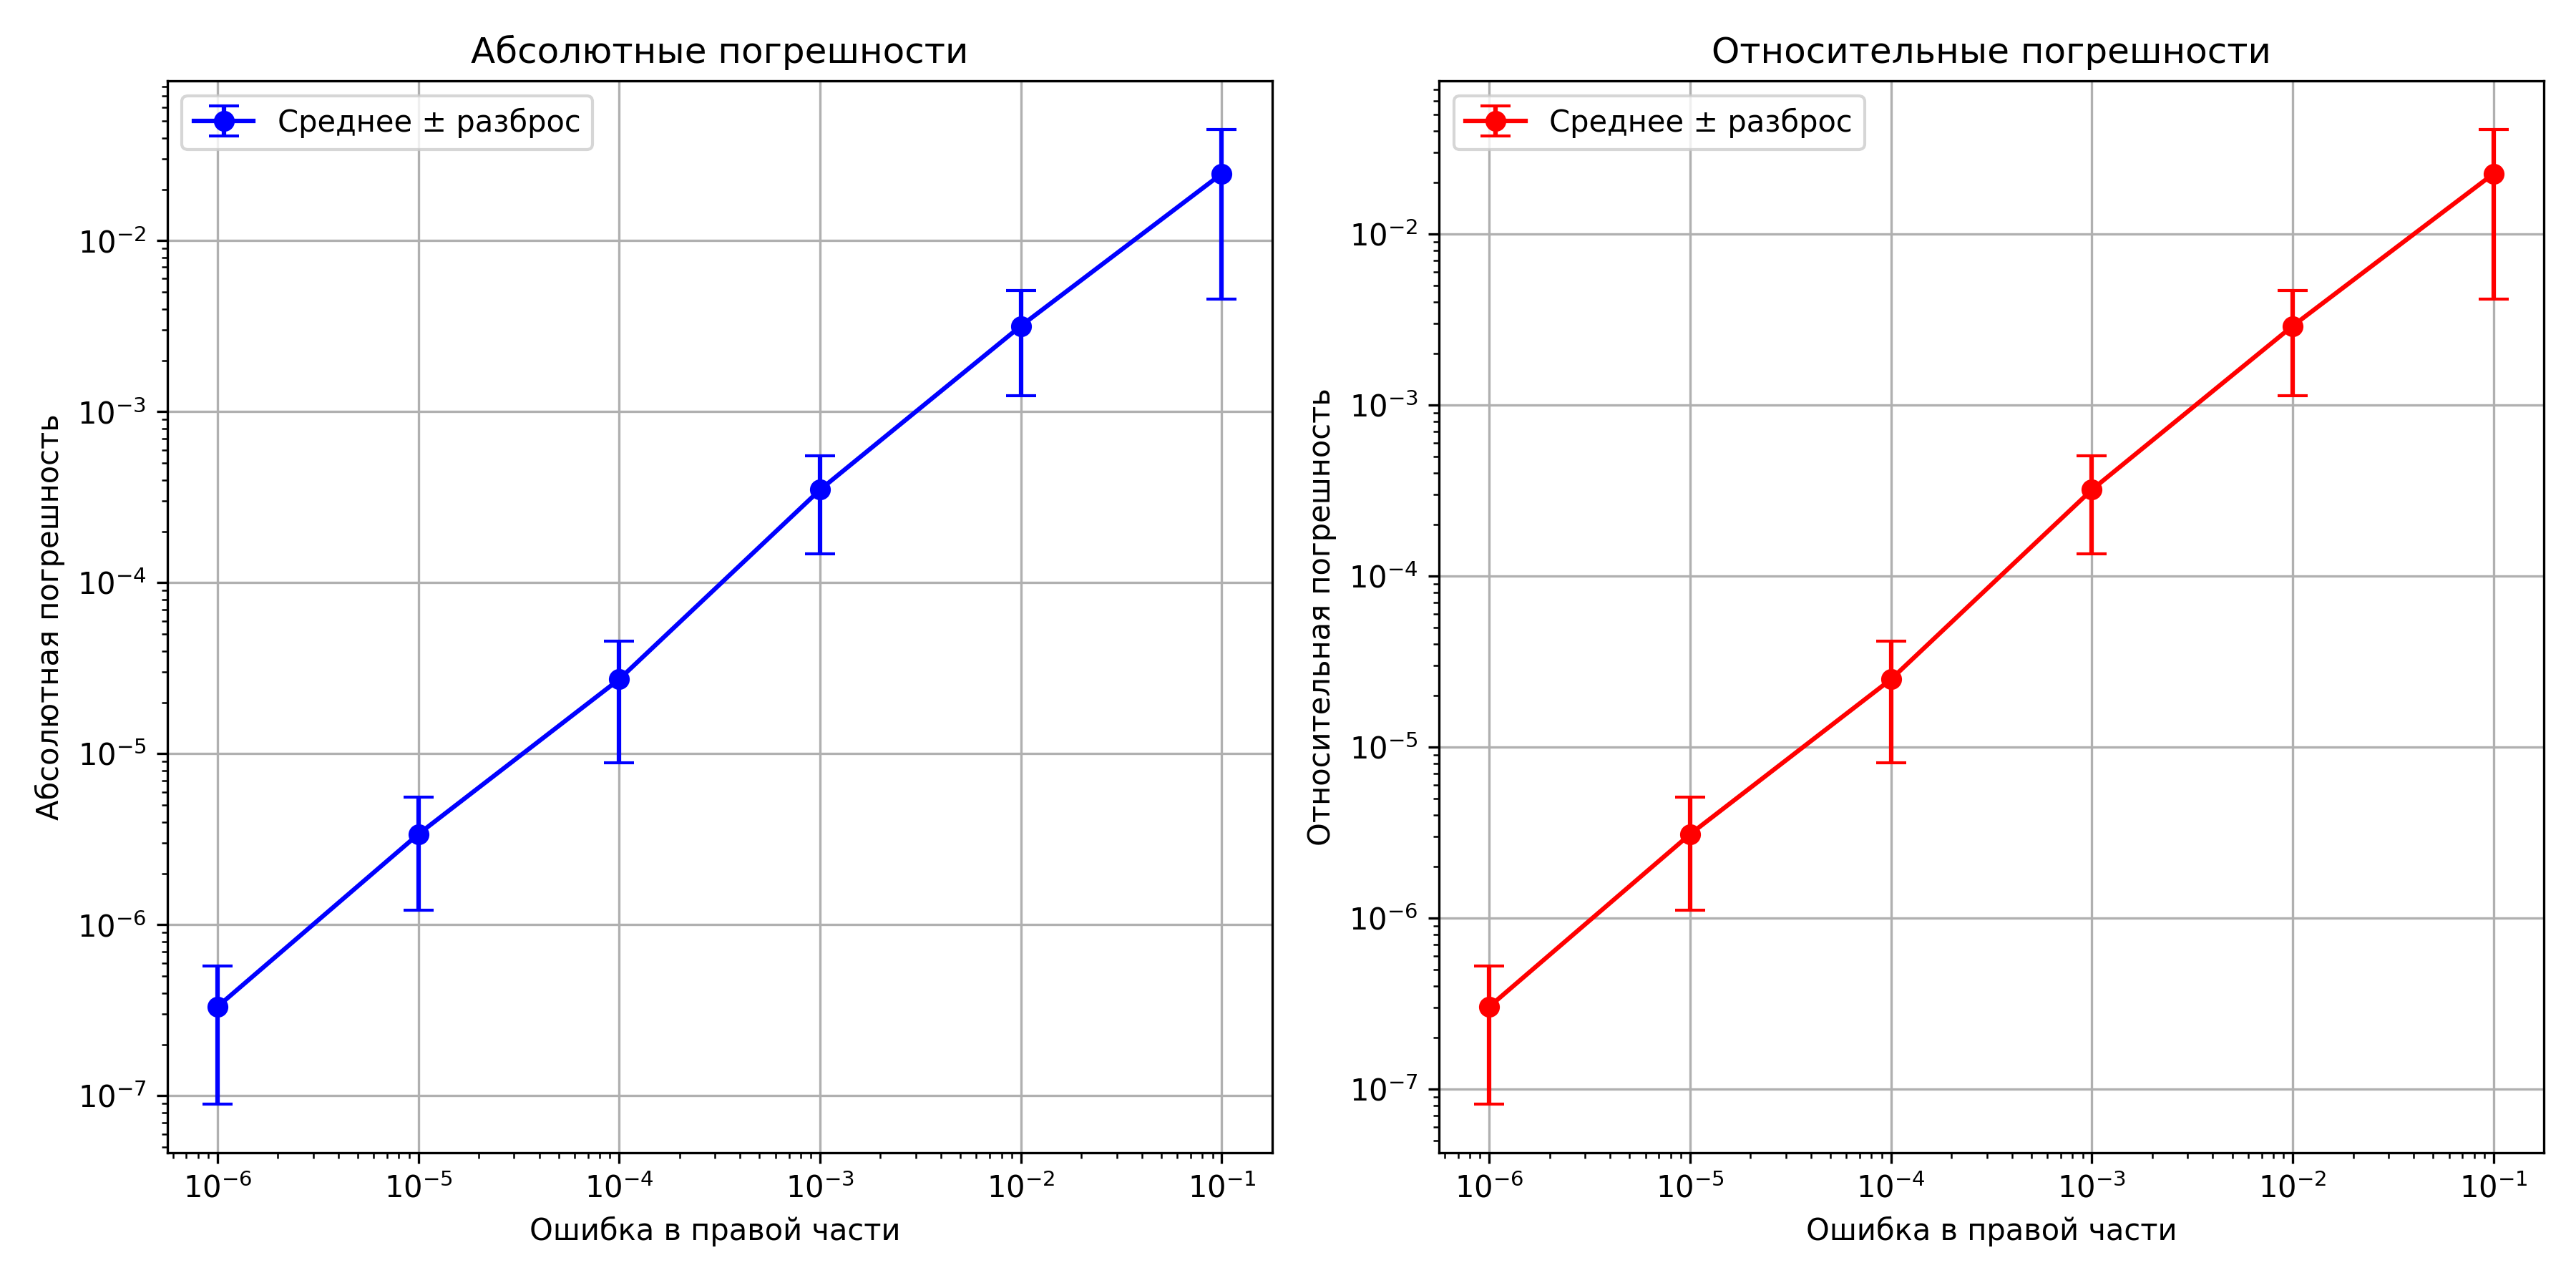
\includegraphics[width=1.0\textwidth]{results.png}
   \caption{Графики зависимости погрешностей от размера ошибки.}
   \label{fig:results}
\end{figure}
\newpage
\section{Вывод}
Симплекс-метод эффективно решает задачи линейного программирования при условии, что все ограничения линейны и функция цели также линейна. Точность решения зависит от точности входных данных, и в случае значительных погрешностей точность результата может существенно снизиться. Разработанное интерактивное приложение на C\# позволяет удобно вводить исходные данные, просматривать каноническую форму задачи, контролировать ход итераций и выполнять вычислительный эксперимент без обращения к исходному коду. Результаты работы подтверждают, что симплекс-метод может быть использован для нахождения оптимальных решений в линейных задачах, при этом вычислительные погрешности должны быть минимизированы для достижения точных и надежных результатов.
\newpage
\begin{table}[h]
   \centering
   \caption{Промежуточные результаты (Размер ошибки: $10^{-6}$)}
   \begin{tabular}{|c|c|c|}
       \hline
       Решение & Абсолютная ошибка & Относительная ошибка \\
       \hline
       $1.1000002$ & $2 \cdot 10^{-7}$ & $2 \cdot 10^{-7}$ \\
       \hline
       $1.1000005$ & $5 \cdot 10^{-7}$ & $5 \cdot 10^{-7}$ \\
       \hline
       $1.1000003$ & $3 \cdot 10^{-7}$ & $3 \cdot 10^{-7}$ \\
       \hline
       $1.1000003$ & $3 \cdot 10^{-7}$ & $3 \cdot 10^{-7}$ \\
       \hline
       $1.1000006$ & $6 \cdot 10^{-7}$ & $6 \cdot 10^{-7}$ \\
       \hline
       $1.1000003$ & $3 \cdot 10^{-7}$ & $3 \cdot 10^{-7}$ \\
       \hline
       $1.0999999$ & $1 \cdot 10^{-7}$ & $1 \cdot 10^{-7}$ \\
       \hline
       $1.1000005$ & $5 \cdot 10^{-7}$ & $5 \cdot 10^{-7}$ \\
       \hline
       $1.0999997$ & $3 \cdot 10^{-7}$ & $2 \cdot 10^{-7}$ \\
       \hline
       $1.1000006$ & $6 \cdot 10^{-7}$ & $5 \cdot 10^{-7}$ \\
       \hline
       $1.1000005$ & $5 \cdot 10^{-7}$ & $5 \cdot 10^{-7}$ \\
       \hline
       $1.1000005$ & $5 \cdot 10^{-7}$ & $5 \cdot 10^{-7}$ \\
       \hline
       $1.1000001$ & $5 \cdot 10^{-8}$ & $5 \cdot 10^{-8}$ \\
       \hline
       $1.1000007$ & $7 \cdot 10^{-7}$ & $6 \cdot 10^{-7}$ \\
       \hline
       $1.0999999$ & $7 \cdot 10^{-8}$ & $6 \cdot 10^{-8}$ \\
       \hline
       $1.0999996$ & $4 \cdot 10^{-7}$ & $3 \cdot 10^{-7}$ \\
       \hline
       $1.1000006$ & $6 \cdot 10^{-7}$ & $5 \cdot 10^{-7}$ \\
       \hline
       $1.0999999$ & $9 \cdot 10^{-8}$ & $8 \cdot 10^{-8}$ \\
       \hline
       $1.1000005$ & $5 \cdot 10^{-7}$ & $5 \cdot 10^{-7}$ \\
       \hline
       $1.1000000$ & $1 \cdot 10^{-8}$ & $1 \cdot 10^{-8}$ \\
       \hline
       $1.1000002$ & $2 \cdot 10^{-7}$ & $2 \cdot 10^{-7}$ \\
       \hline
       $1.1000002$ & $2 \cdot 10^{-7}$ & $2 \cdot 10^{-7}$ \\
       \hline
       $1.1000001$ & $9 \cdot 10^{-8}$ & $9 \cdot 10^{-8}$ \\
       \hline
       $1.1000006$ & $6 \cdot 10^{-7}$ & $5 \cdot 10^{-7}$ \\
       \hline
       $1.0999999$ & $1 \cdot 10^{-7}$ & $1 \cdot 10^{-7}$ \\
       \hline
       $1.1000003$ & $3 \cdot 10^{-7}$ & $3 \cdot 10^{-7}$ \\
       \hline
       $1.1000005$ & $5 \cdot 10^{-7}$ & $5 \cdot 10^{-7}$ \\
       \hline
       $1.0999996$ & $4 \cdot 10^{-7}$ & $4 \cdot 10^{-7}$ \\
       \hline
       $1.1000008$ & $8 \cdot 10^{-7}$ & $8 \cdot 10^{-7}$ \\
       \hline
       $1.1000001$ & $6 \cdot 10^{-8}$ & $5 \cdot 10^{-8}$ \\
       \hline
       $1.0999994$ & $6 \cdot 10^{-7}$ & $6 \cdot 10^{-7}$ \\
       \hline
       $1.1000002$ & $2 \cdot 10^{-7}$ & $2 \cdot 10^{-7}$ \\
       \hline
       $1.0999999$ & $9 \cdot 10^{-8}$ & $8 \cdot 10^{-8}$ \\
       \hline
       $1.0999996$ & $4 \cdot 10^{-7}$ & $3 \cdot 10^{-7}$ \\
       \hline
       $1.1000004$ & $4 \cdot 10^{-7}$ & $3 \cdot 10^{-7}$ \\
       \hline
       $1.1000000$ & $1 \cdot 10^{-8}$ & $1 \cdot 10^{-8}$ \\
       \hline
       $1.1000000$ & $5 \cdot 10^{-8}$ & $4 \cdot 10^{-8}$ \\
       \hline
       $1.0999999$ & $8 \cdot 10^{-8}$ & $8 \cdot 10^{-8}$ \\
       \hline
       $1.0999999$ & $1 \cdot 10^{-7}$ & $1 \cdot 10^{-7}$ \\
       \hline
       $1.1000004$ & $4 \cdot 10^{-7}$ & $4 \cdot 10^{-7}$ \\
       \hline
       $1.1000007$ & $7 \cdot 10^{-7}$ & $7 \cdot 10^{-7}$ \\
       \hline
       $1.1000000$ & $4 \cdot 10^{-9}$ & $4 \cdot 10^{-9}$ \\
       \hline
       $1.0999998$ & $2 \cdot 10^{-7}$ & $2 \cdot 10^{-7}$ \\
       \hline
       $1.1000010$ & $10 \cdot 10^{-7}$ & $9 \cdot 10^{-7}$ \\
       \hline
       $1.0999999$ & $1 \cdot 10^{-7}$ & $1 \cdot 10^{-7}$ \\
       \hline
   \end{tabular}
\end{table}


\begin{table}[h]
   \centering
   \caption{Промежуточные результаты (Размер ошибки: $10^{-5}$)}
   \begin{tabular}{|c|c|c|}
       \hline
       Решение & Абсолютная ошибка & Относительная ошибка \\
       \hline
       $1.100004$ & $4 \cdot 10^{-6}$ & $4 \cdot 10^{-6}$ \\
       \hline
       $1.100004$ & $4 \cdot 10^{-6}$ & $4 \cdot 10^{-6}$ \\
       \hline
       $1.099998$ & $2 \cdot 10^{-6}$ & $2 \cdot 10^{-6}$ \\
       \hline
       $1.100007$ & $7 \cdot 10^{-6}$ & $6 \cdot 10^{-6}$ \\
       \hline
       $1.100004$ & $4 \cdot 10^{-6}$ & $4 \cdot 10^{-6}$ \\
       \hline
       $1.100003$ & $3 \cdot 10^{-6}$ & $3 \cdot 10^{-6}$ \\
       \hline
       $1.099998$ & $2 \cdot 10^{-6}$ & $2 \cdot 10^{-6}$ \\
       \hline
       $1.099995$ & $5 \cdot 10^{-6}$ & $5 \cdot 10^{-6}$ \\
       \hline
       $1.099999$ & $1 \cdot 10^{-6}$ & $1 \cdot 10^{-6}$ \\
       \hline
       $1.100005$ & $5 \cdot 10^{-6}$ & $4 \cdot 10^{-6}$ \\
       \hline
       $1.100004$ & $4 \cdot 10^{-6}$ & $4 \cdot 10^{-6}$ \\
       \hline
       $1.100001$ & $1 \cdot 10^{-6}$ & $1 \cdot 10^{-6}$ \\
       \hline
       $1.100006$ & $6 \cdot 10^{-6}$ & $5 \cdot 10^{-6}$ \\
       \hline
       $1.100006$ & $6 \cdot 10^{-6}$ & $5 \cdot 10^{-6}$ \\
       \hline
       $1.100005$ & $5 \cdot 10^{-6}$ & $4 \cdot 10^{-6}$ \\
       \hline
       $1.100006$ & $6 \cdot 10^{-6}$ & $6 \cdot 10^{-6}$ \\
       \hline
       $1.100001$ & $8 \cdot 10^{-7}$ & $8 \cdot 10^{-7}$ \\
       \hline
       $1.100000$ & $2 \cdot 10^{-7}$ & $2 \cdot 10^{-7}$ \\
       \hline
       $1.099996$ & $4 \cdot 10^{-6}$ & $4 \cdot 10^{-6}$ \\
       \hline
       $1.099999$ & $1 \cdot 10^{-6}$ & $9 \cdot 10^{-7}$ \\
       \hline
       $1.100001$ & $1 \cdot 10^{-6}$ & $1 \cdot 10^{-6}$ \\
       \hline
       $1.100006$ & $6 \cdot 10^{-6}$ & $6 \cdot 10^{-6}$ \\
       \hline
       $1.100004$ & $4 \cdot 10^{-6}$ & $3 \cdot 10^{-6}$ \\
       \hline
       $1.099999$ & $1 \cdot 10^{-6}$ & $1 \cdot 10^{-6}$ \\
       \hline
       $1.100000$ & $3 \cdot 10^{-7}$ & $3 \cdot 10^{-7}$ \\
       \hline
       $1.100008$ & $8 \cdot 10^{-6}$ & $7 \cdot 10^{-6}$ \\
       \hline
       $1.100000$ & $4 \cdot 10^{-7}$ & $4 \cdot 10^{-7}$ \\
       \hline
       $1.100007$ & $7 \cdot 10^{-6}$ & $6 \cdot 10^{-6}$ \\
       \hline
       $1.100006$ & $6 \cdot 10^{-6}$ & $6 \cdot 10^{-6}$ \\
       \hline
       $1.099999$ & $7 \cdot 10^{-7}$ & $6 \cdot 10^{-7}$ \\
       \hline
       $1.099996$ & $4 \cdot 10^{-6}$ & $3 \cdot 10^{-6}$ \\
       \hline
       $1.099996$ & $4 \cdot 10^{-6}$ & $3 \cdot 10^{-6}$ \\
       \hline
       $1.100006$ & $6 \cdot 10^{-6}$ & $6 \cdot 10^{-6}$ \\
       \hline
       $1.099999$ & $7 \cdot 10^{-7}$ & $6 \cdot 10^{-7}$ \\
       \hline
       $1.100002$ & $2 \cdot 10^{-6}$ & $2 \cdot 10^{-6}$ \\
       \hline
       $1.100004$ & $4 \cdot 10^{-6}$ & $4 \cdot 10^{-6}$ \\
       \hline
       $1.100003$ & $3 \cdot 10^{-6}$ & $3 \cdot 10^{-6}$ \\
       \hline
       $1.099998$ & $2 \cdot 10^{-6}$ & $1 \cdot 10^{-6}$ \\
       \hline
       $1.100004$ & $4 \cdot 10^{-6}$ & $4 \cdot 10^{-6}$ \\
       \hline
       $1.100006$ & $6 \cdot 10^{-6}$ & $5 \cdot 10^{-6}$ \\
       \hline
       $1.099994$ & $6 \cdot 10^{-6}$ & $5 \cdot 10^{-6}$ \\
       \hline
       $1.100000$ & $2 \cdot 10^{-7}$ & $1 \cdot 10^{-7}$ \\
       \hline
       $1.099999$ & $7 \cdot 10^{-7}$ & $6 \cdot 10^{-7}$ \\
       \hline
       $1.100003$ & $3 \cdot 10^{-6}$ & $2 \cdot 10^{-6}$ \\
       \hline
       $1.099998$ & $2 \cdot 10^{-6}$ & $1 \cdot 10^{-6}$ \\
       \hline
   \end{tabular}
\end{table}


\begin{table}[h]
   \centering
   \caption{Промежуточные результаты (Размер ошибки: $10^{-4}$)}
   \begin{tabular}{|c|c|c|}
       \hline
       Решение & Абсолютная ошибка & Относительная ошибка \\
       \hline
       $1.10005$ & $5 \cdot 10^{-5}$ & $4 \cdot 10^{-5}$ \\
       \hline
       $1.10001$ & $10 \cdot 10^{-6}$ & $9 \cdot 10^{-6}$ \\
       \hline
       $1.10002$ & $2 \cdot 10^{-5}$ & $2 \cdot 10^{-5}$ \\
       \hline
       $1.09997$ & $3 \cdot 10^{-5}$ & $3 \cdot 10^{-5}$ \\
       \hline
       $1.10001$ & $1 \cdot 10^{-5}$ & $1 \cdot 10^{-5}$ \\
       \hline
       $1.09997$ & $3 \cdot 10^{-5}$ & $2 \cdot 10^{-5}$ \\
       \hline
       $1.09999$ & $7 \cdot 10^{-6}$ & $6 \cdot 10^{-6}$ \\
       \hline
       $1.10002$ & $2 \cdot 10^{-5}$ & $2 \cdot 10^{-5}$ \\
       \hline
       $1.10003$ & $3 \cdot 10^{-5}$ & $3 \cdot 10^{-5}$ \\
       \hline
       $1.10000$ & $2 \cdot 10^{-7}$ & $2 \cdot 10^{-7}$ \\
       \hline
       $1.09999$ & $1 \cdot 10^{-5}$ & $1 \cdot 10^{-5}$ \\
       \hline
       $1.10004$ & $4 \cdot 10^{-5}$ & $3 \cdot 10^{-5}$ \\
       \hline
       $1.10006$ & $6 \cdot 10^{-5}$ & $5 \cdot 10^{-5}$ \\
       \hline
       $1.09997$ & $3 \cdot 10^{-5}$ & $3 \cdot 10^{-5}$ \\
       \hline
       $1.09998$ & $2 \cdot 10^{-5}$ & $1 \cdot 10^{-5}$ \\
       \hline
       $1.10005$ & $5 \cdot 10^{-5}$ & $5 \cdot 10^{-5}$ \\
       \hline
       $1.10000$ & $5 \cdot 10^{-6}$ & $4 \cdot 10^{-6}$ \\
       \hline
       $1.10003$ & $3 \cdot 10^{-5}$ & $2 \cdot 10^{-5}$ \\
       \hline
       $1.10003$ & $3 \cdot 10^{-5}$ & $3 \cdot 10^{-5}$ \\
       \hline
       $1.10000$ & $5 \cdot 10^{-6}$ & $4 \cdot 10^{-6}$ \\
       \hline
       $1.10006$ & $6 \cdot 10^{-5}$ & $6 \cdot 10^{-5}$ \\
       \hline
       $1.10005$ & $5 \cdot 10^{-5}$ & $4 \cdot 10^{-5}$ \\
       \hline
       $1.10000$ & $4 \cdot 10^{-6}$ & $4 \cdot 10^{-6}$ \\
       \hline
       $1.09994$ & $6 \cdot 10^{-5}$ & $6 \cdot 10^{-5}$ \\
       \hline
       $1.09999$ & $7 \cdot 10^{-6}$ & $6 \cdot 10^{-6}$ \\
       \hline
       $1.10005$ & $5 \cdot 10^{-5}$ & $5 \cdot 10^{-5}$ \\
       \hline
       $1.09996$ & $4 \cdot 10^{-5}$ & $4 \cdot 10^{-5}$ \\
       \hline
       $1.10005$ & $5 \cdot 10^{-5}$ & $4 \cdot 10^{-5}$ \\
       \hline
       $1.09999$ & $5 \cdot 10^{-6}$ & $5 \cdot 10^{-6}$ \\
       \hline
       $1.10000$ & $1 \cdot 10^{-6}$ & $1 \cdot 10^{-6}$ \\
       \hline
       $1.10000$ & $2 \cdot 10^{-6}$ & $2 \cdot 10^{-6}$ \\
       \hline
       $1.10006$ & $6 \cdot 10^{-5}$ & $6 \cdot 10^{-5}$ \\
       \hline
       $1.10003$ & $3 \cdot 10^{-5}$ & $3 \cdot 10^{-5}$ \\
       \hline
       $1.09998$ & $2 \cdot 10^{-5}$ & $2 \cdot 10^{-5}$ \\
       \hline
       $1.10004$ & $4 \cdot 10^{-5}$ & $4 \cdot 10^{-5}$ \\
       \hline
       $1.10004$ & $4 \cdot 10^{-5}$ & $3 \cdot 10^{-5}$ \\
       \hline
       $1.10000$ & $2 \cdot 10^{-6}$ & $2 \cdot 10^{-6}$ \\
       \hline
       $1.09995$ & $5 \cdot 10^{-5}$ & $5 \cdot 10^{-5}$ \\
       \hline
       $1.10003$ & $3 \cdot 10^{-5}$ & $3 \cdot 10^{-5}$ \\
       \hline
       $1.10002$ & $2 \cdot 10^{-5}$ & $2 \cdot 10^{-5}$ \\
       \hline
       $1.10003$ & $3 \cdot 10^{-5}$ & $3 \cdot 10^{-5}$ \\
       \hline
       $1.10003$ & $3 \cdot 10^{-5}$ & $3 \cdot 10^{-5}$ \\
       \hline
       $1.10002$ & $2 \cdot 10^{-5}$ & $1 \cdot 10^{-5}$ \\
       \hline
       $1.10002$ & $2 \cdot 10^{-5}$ & $2 \cdot 10^{-5}$ \\
       \hline
       $1.09999$ & $1 \cdot 10^{-5}$ & $1 \cdot 10^{-5}$ \\
       \hline
   \end{tabular}
\end{table}


\begin{table}[h]
   \centering
   \caption{Промежуточные результаты (Размер ошибки: $10^{-3}$)}
   \begin{tabular}{|c|c|c|}
       \hline
       Решение & Абсолютная ошибка & Относительная ошибка \\
       \hline
       $1.0996$ & $4 \cdot 10^{-4}$ & $4 \cdot 10^{-4}$ \\
       \hline
       $1.1004$ & $4 \cdot 10^{-4}$ & $4 \cdot 10^{-4}$ \\
       \hline
       $1.1003$ & $3 \cdot 10^{-4}$ & $3 \cdot 10^{-4}$ \\
       \hline
       $1.1002$ & $2 \cdot 10^{-4}$ & $2 \cdot 10^{-4}$ \\
       \hline
       $1.1001$ & $1 \cdot 10^{-4}$ & $1 \cdot 10^{-4}$ \\
       \hline
       $1.1002$ & $2 \cdot 10^{-4}$ & $2 \cdot 10^{-4}$ \\
       \hline
       $1.0997$ & $3 \cdot 10^{-4}$ & $2 \cdot 10^{-4}$ \\
       \hline
       $1.1001$ & $1 \cdot 10^{-4}$ & $1 \cdot 10^{-4}$ \\
       \hline
       $1.0999$ & $6 \cdot 10^{-5}$ & $6 \cdot 10^{-5}$ \\
       \hline
       $1.1007$ & $7 \cdot 10^{-4}$ & $6 \cdot 10^{-4}$ \\
       \hline
       $1.0999$ & $8 \cdot 10^{-5}$ & $7 \cdot 10^{-5}$ \\
       \hline
       $1.1006$ & $6 \cdot 10^{-4}$ & $5 \cdot 10^{-4}$ \\
       \hline
       $1.1002$ & $2 \cdot 10^{-4}$ & $1 \cdot 10^{-4}$ \\
       \hline
       $1.1003$ & $3 \cdot 10^{-4}$ & $3 \cdot 10^{-4}$ \\
       \hline
       $1.1004$ & $4 \cdot 10^{-4}$ & $4 \cdot 10^{-4}$ \\
       \hline
       $1.0994$ & $6 \cdot 10^{-4}$ & $6 \cdot 10^{-4}$ \\
       \hline
       $1.1006$ & $6 \cdot 10^{-4}$ & $5 \cdot 10^{-4}$ \\
       \hline
       $1.1004$ & $4 \cdot 10^{-4}$ & $3 \cdot 10^{-4}$ \\
       \hline
       $1.0997$ & $3 \cdot 10^{-4}$ & $3 \cdot 10^{-4}$ \\
       \hline
       $1.1006$ & $6 \cdot 10^{-4}$ & $5 \cdot 10^{-4}$ \\
       \hline
       $1.1005$ & $5 \cdot 10^{-4}$ & $4 \cdot 10^{-4}$ \\
       \hline
       $1.0996$ & $4 \cdot 10^{-4}$ & $4 \cdot 10^{-4}$ \\
       \hline
       $1.0998$ & $2 \cdot 10^{-4}$ & $2 \cdot 10^{-4}$ \\
       \hline
       $1.0997$ & $3 \cdot 10^{-4}$ & $3 \cdot 10^{-4}$ \\
       \hline
       $1.1001$ & $8 \cdot 10^{-5}$ & $8 \cdot 10^{-5}$ \\
       \hline
       $1.1001$ & $9 \cdot 10^{-5}$ & $8 \cdot 10^{-5}$ \\
       \hline
       $1.1003$ & $3 \cdot 10^{-4}$ & $2 \cdot 10^{-4}$ \\
       \hline
       $1.1001$ & $7 \cdot 10^{-5}$ & $6 \cdot 10^{-5}$ \\
       \hline
       $1.1002$ & $2 \cdot 10^{-4}$ & $2 \cdot 10^{-4}$ \\
       \hline
       $1.1006$ & $6 \cdot 10^{-4}$ & $5 \cdot 10^{-4}$ \\
       \hline
       $1.1006$ & $6 \cdot 10^{-4}$ & $6 \cdot 10^{-4}$ \\
       \hline
       $1.1000$ & $5 \cdot 10^{-5}$ & $4 \cdot 10^{-5}$ \\
       \hline
       $1.1007$ & $7 \cdot 10^{-4}$ & $7 \cdot 10^{-4}$ \\
       \hline
       $1.0993$ & $7 \cdot 10^{-4}$ & $7 \cdot 10^{-4}$ \\
       \hline
       $1.1006$ & $6 \cdot 10^{-4}$ & $5 \cdot 10^{-4}$ \\
       \hline
       $1.1005$ & $5 \cdot 10^{-4}$ & $5 \cdot 10^{-4}$ \\
       \hline
       $1.1004$ & $4 \cdot 10^{-4}$ & $3 \cdot 10^{-4}$ \\
       \hline
       $1.1002$ & $2 \cdot 10^{-4}$ & $2 \cdot 10^{-4}$ \\
       \hline
       $1.1001$ & $1 \cdot 10^{-4}$ & $1 \cdot 10^{-4}$ \\
       \hline
       $1.1002$ & $2 \cdot 10^{-4}$ & $2 \cdot 10^{-4}$ \\
       \hline
       $1.1005$ & $5 \cdot 10^{-4}$ & $5 \cdot 10^{-4}$ \\
       \hline
       $1.1004$ & $4 \cdot 10^{-4}$ & $4 \cdot 10^{-4}$ \\
       \hline
       $1.1007$ & $7 \cdot 10^{-4}$ & $6 \cdot 10^{-4}$ \\
       \hline
       $1.1002$ & $2 \cdot 10^{-4}$ & $2 \cdot 10^{-4}$ \\
       \hline
       $1.1004$ & $4 \cdot 10^{-4}$ & $4 \cdot 10^{-4}$ \\
       \hline
   \end{tabular}
\end{table}


\begin{table}[h]
   \centering
   \caption{Промежуточные результаты (Размер ошибки: $10^{-2}$)}
   \begin{tabular}{|c|c|c|}
       \hline
       Решение & Абсолютная ошибка & Относительная ошибка \\
       \hline
       $1.105$ & $5 \cdot 10^{-3}$ & $4 \cdot 10^{-3}$ \\
       \hline
       $1.102$ & $2 \cdot 10^{-3}$ & $2 \cdot 10^{-3}$ \\
       \hline
       $1.104$ & $4 \cdot 10^{-3}$ & $4 \cdot 10^{-3}$ \\
       \hline
       $1.098$ & $2 \cdot 10^{-3}$ & $2 \cdot 10^{-3}$ \\
       \hline
       $1.106$ & $6 \cdot 10^{-3}$ & $6 \cdot 10^{-3}$ \\
       \hline
       $1.103$ & $3 \cdot 10^{-3}$ & $3 \cdot 10^{-3}$ \\
       \hline
       $1.102$ & $2 \cdot 10^{-3}$ & $2 \cdot 10^{-3}$ \\
       \hline
       $1.104$ & $4 \cdot 10^{-3}$ & $4 \cdot 10^{-3}$ \\
       \hline
       $1.099$ & $1 \cdot 10^{-3}$ & $1 \cdot 10^{-3}$ \\
       \hline
       $1.108$ & $8 \cdot 10^{-3}$ & $7 \cdot 10^{-3}$ \\
       \hline
       $1.105$ & $5 \cdot 10^{-3}$ & $5 \cdot 10^{-3}$ \\
       \hline
       $1.105$ & $5 \cdot 10^{-3}$ & $5 \cdot 10^{-3}$ \\
       \hline
       $1.098$ & $2 \cdot 10^{-3}$ & $2 \cdot 10^{-3}$ \\
       \hline
       $1.093$ & $7 \cdot 10^{-3}$ & $6 \cdot 10^{-3}$ \\
       \hline
       $1.104$ & $4 \cdot 10^{-3}$ & $4 \cdot 10^{-3}$ \\
       \hline
       $1.099$ & $9 \cdot 10^{-4}$ & $8 \cdot 10^{-4}$ \\
       \hline
       $1.094$ & $6 \cdot 10^{-3}$ & $5 \cdot 10^{-3}$ \\
       \hline
       $1.103$ & $3 \cdot 10^{-3}$ & $3 \cdot 10^{-3}$ \\
       \hline
       $1.102$ & $2 \cdot 10^{-3}$ & $2 \cdot 10^{-3}$ \\
       \hline
       $1.101$ & $1 \cdot 10^{-3}$ & $10 \cdot 10^{-4}$ \\
       \hline
       $1.098$ & $2 \cdot 10^{-3}$ & $2 \cdot 10^{-3}$ \\
       \hline
       $1.103$ & $3 \cdot 10^{-3}$ & $2 \cdot 10^{-3}$ \\
       \hline
       $1.103$ & $3 \cdot 10^{-3}$ & $2 \cdot 10^{-3}$ \\
       \hline
       $1.106$ & $6 \cdot 10^{-3}$ & $5 \cdot 10^{-3}$ \\
       \hline
       $1.104$ & $4 \cdot 10^{-3}$ & $4 \cdot 10^{-3}$ \\
       \hline
       $1.102$ & $2 \cdot 10^{-3}$ & $2 \cdot 10^{-3}$ \\
       \hline
       $1.100$ & $1 \cdot 10^{-4}$ & $1 \cdot 10^{-4}$ \\
       \hline
       $1.098$ & $2 \cdot 10^{-3}$ & $2 \cdot 10^{-3}$ \\
       \hline
       $1.101$ & $6 \cdot 10^{-4}$ & $6 \cdot 10^{-4}$ \\
       \hline
       $1.105$ & $5 \cdot 10^{-3}$ & $4 \cdot 10^{-3}$ \\
       \hline
       $1.098$ & $2 \cdot 10^{-3}$ & $2 \cdot 10^{-3}$ \\
       \hline
       $1.104$ & $4 \cdot 10^{-3}$ & $3 \cdot 10^{-3}$ \\
       \hline
       $1.102$ & $2 \cdot 10^{-3}$ & $1 \cdot 10^{-3}$ \\
       \hline
       $1.104$ & $4 \cdot 10^{-3}$ & $3 \cdot 10^{-3}$ \\
       \hline
       $1.101$ & $7 \cdot 10^{-4}$ & $6 \cdot 10^{-4}$ \\
       \hline
       $1.106$ & $6 \cdot 10^{-3}$ & $6 \cdot 10^{-3}$ \\
       \hline
       $1.104$ & $4 \cdot 10^{-3}$ & $3 \cdot 10^{-3}$ \\
       \hline
       $1.104$ & $4 \cdot 10^{-3}$ & $3 \cdot 10^{-3}$ \\
       \hline
       $1.107$ & $7 \cdot 10^{-3}$ & $6 \cdot 10^{-3}$ \\
       \hline
       $1.099$ & $5 \cdot 10^{-4}$ & $5 \cdot 10^{-4}$ \\
       \hline
       $1.104$ & $4 \cdot 10^{-3}$ & $4 \cdot 10^{-3}$ \\
       \hline
       $1.099$ & $9 \cdot 10^{-4}$ & $8 \cdot 10^{-4}$ \\
       \hline
       $1.098$ & $2 \cdot 10^{-3}$ & $1 \cdot 10^{-3}$ \\
       \hline
       $1.102$ & $2 \cdot 10^{-3}$ & $2 \cdot 10^{-3}$ \\
       \hline
       $1.102$ & $2 \cdot 10^{-3}$ & $2 \cdot 10^{-3}$ \\
       \hline
   \end{tabular}
\end{table}


\begin{table}[h]
   \centering
   \caption{Промежуточные результаты (Размер ошибки: $10^{-1}$)}
   \begin{tabular}{|c|c|c|}
       \hline
       Решение & Абсолютная ошибка & Относительная ошибка \\
       \hline
       $1.14$ & $4 \cdot 10^{-2}$ & $4 \cdot 10^{-2}$ \\
       \hline
       $1.12$ & $2 \cdot 10^{-2}$ & $2 \cdot 10^{-2}$ \\
       \hline
       $1.16$ & $6 \cdot 10^{-2}$ & $6 \cdot 10^{-2}$ \\
       \hline
       $1.17$ & $7 \cdot 10^{-2}$ & $6 \cdot 10^{-2}$ \\
       \hline
       $1.05$ & $5 \cdot 10^{-2}$ & $5 \cdot 10^{-2}$ \\
       \hline
       $1.14$ & $4 \cdot 10^{-2}$ & $4 \cdot 10^{-2}$ \\
       \hline
       $1.08$ & $2 \cdot 10^{-2}$ & $2 \cdot 10^{-2}$ \\
       \hline
       $1.11$ & $9 \cdot 10^{-3}$ & $8 \cdot 10^{-3}$ \\
       \hline
       $1.11$ & $7 \cdot 10^{-3}$ & $7 \cdot 10^{-3}$ \\
       \hline
       $1.09$ & $7 \cdot 10^{-3}$ & $7 \cdot 10^{-3}$ \\
       \hline
       $1.10$ & $9 \cdot 10^{-5}$ & $8 \cdot 10^{-5}$ \\
       \hline
       $1.13$ & $3 \cdot 10^{-2}$ & $3 \cdot 10^{-2}$ \\
       \hline
       $1.13$ & $3 \cdot 10^{-2}$ & $3 \cdot 10^{-2}$ \\
       \hline
       $1.12$ & $2 \cdot 10^{-2}$ & $2 \cdot 10^{-2}$ \\
       \hline
       $1.11$ & $1 \cdot 10^{-2}$ & $9 \cdot 10^{-3}$ \\
       \hline
       $1.09$ & $8 \cdot 10^{-3}$ & $7 \cdot 10^{-3}$ \\
       \hline
       $1.08$ & $2 \cdot 10^{-2}$ & $2 \cdot 10^{-2}$ \\
       \hline
       $1.14$ & $4 \cdot 10^{-2}$ & $4 \cdot 10^{-2}$ \\
       \hline
       $1.09$ & $9 \cdot 10^{-3}$ & $9 \cdot 10^{-3}$ \\
       \hline
       $1.19$ & $9 \cdot 10^{-2}$ & $8 \cdot 10^{-2}$ \\
       \hline
       $1.14$ & $4 \cdot 10^{-2}$ & $3 \cdot 10^{-2}$ \\
       \hline
       $1.12$ & $2 \cdot 10^{-2}$ & $2 \cdot 10^{-2}$ \\
       \hline
       $1.13$ & $3 \cdot 10^{-2}$ & $3 \cdot 10^{-2}$ \\
       \hline
       $1.12$ & $2 \cdot 10^{-2}$ & $2 \cdot 10^{-2}$ \\
       \hline
       $1.11$ & $1 \cdot 10^{-2}$ & $9 \cdot 10^{-3}$ \\
       \hline
       $1.06$ & $4 \cdot 10^{-2}$ & $4 \cdot 10^{-2}$ \\
       \hline
       $1.11$ & $1 \cdot 10^{-2}$ & $1 \cdot 10^{-2}$ \\
       \hline
       $1.10$ & $10 \cdot 10^{-4}$ & $9 \cdot 10^{-4}$ \\
       \hline
       $1.13$ & $3 \cdot 10^{-2}$ & $3 \cdot 10^{-2}$ \\
       \hline
       $1.12$ & $2 \cdot 10^{-2}$ & $2 \cdot 10^{-2}$ \\
       \hline
       $1.11$ & $8 \cdot 10^{-3}$ & $7 \cdot 10^{-3}$ \\
       \hline
       $1.12$ & $2 \cdot 10^{-2}$ & $2 \cdot 10^{-2}$ \\
       \hline
       $1.10$ & $2 \cdot 10^{-3}$ & $2 \cdot 10^{-3}$ \\
       \hline
       $1.10$ & $2 \cdot 10^{-3}$ & $2 \cdot 10^{-3}$ \\
       \hline
       $1.09$ & $1 \cdot 10^{-2}$ & $1 \cdot 10^{-2}$ \\
       \hline
       $1.14$ & $4 \cdot 10^{-2}$ & $4 \cdot 10^{-2}$ \\
       \hline
       $1.12$ & $2 \cdot 10^{-2}$ & $1 \cdot 10^{-2}$ \\
       \hline
       $1.08$ & $2 \cdot 10^{-2}$ & $1 \cdot 10^{-2}$ \\
       \hline
       $1.17$ & $7 \cdot 10^{-2}$ & $6 \cdot 10^{-2}$ \\
       \hline
       $1.08$ & $2 \cdot 10^{-2}$ & $2 \cdot 10^{-2}$ \\
       \hline
       $1.09$ & $6 \cdot 10^{-3}$ & $5 \cdot 10^{-3}$ \\
       \hline
       $1.12$ & $2 \cdot 10^{-2}$ & $2 \cdot 10^{-2}$ \\
       \hline
       $1.14$ & $4 \cdot 10^{-2}$ & $3 \cdot 10^{-2}$ \\
       \hline
       $1.10$ & $8 \cdot 10^{-4}$ & $7 \cdot 10^{-4}$ \\
       \hline
       $1.12$ & $2 \cdot 10^{-2}$ & $2 \cdot 10^{-2}$ \\
       \hline
   \end{tabular}
\end{table}


\begin{table}[h]
   \centering
   \caption{Средние значения и стандартные отклонения для различных размеров ошибок}
   \begin{tabular}{|c|c|c|c|c|}
       \hline
       Размер ошибки & $\overline{\Delta_{abs}}$ & $\sigma_{abs}$ & $\overline{\Delta_{rel}}$ & $\sigma_{rel}$ \\
       \hline
       $10^{-6}$ & $3.3 \cdot 10^{-7}$ & $2.4 \cdot 10^{-7}$ & $3.0 \cdot 10^{-7}$ & $2.2 \cdot 10^{-7}$ \\
       \hline
       $10^{-5}$ & $3.4 \cdot 10^{-6}$ & $2.2 \cdot 10^{-6}$ & $3.1 \cdot 10^{-6}$ & $2.0 \cdot 10^{-6}$ \\
       \hline
       $10^{-4}$ & $2.7 \cdot 10^{-5}$ & $1.8 \cdot 10^{-5}$ & $2.5 \cdot 10^{-5}$ & $1.7 \cdot 10^{-5}$ \\
       \hline
       $10^{-3}$ & $3.5 \cdot 10^{-4}$ & $2.0 \cdot 10^{-4}$ & $3.2 \cdot 10^{-4}$ & $1.8 \cdot 10^{-4}$ \\
       \hline
       $10^{-2}$ & $3.2 \cdot 10^{-3}$ & $1.9 \cdot 10^{-3}$ & $2.9 \cdot 10^{-3}$ & $1.8 \cdot 10^{-3}$ \\
       \hline
       $10^{-1}$ & $2.5 \cdot 10^{-2}$ & $2.0 \cdot 10^{-2}$ & $2.2 \cdot 10^{-2}$ & $1.8 \cdot 10^{-2}$ \\
       \hline
   \end{tabular}
\end{table}




% \newpage
% \lstinputlisting[caption={Реализация симплекс метода}]{../main.c}
